% \iffalse meta-comment
%
% Copyright (C) 2019 by Zangwei Zheng <zhengzangw@gmail.com>
%
% This file may be distributed and/or modified under the conditions of
% the LaTeX Project Public License, either version 1.3c of this license
% or (at your option) any later version. The latest version of this 
% license is in:
%
%   http://www.latex-project.org/lppl.txt
%
% and version 1.3c or later is part of all distributions of LaTeX
% version 2005/12/01 or later.
%
% \fi
%
% \iffalse
%<*driver>
\ProvidesFile{njurepo.dtx}[2019/01/29 1.0.1 Nanjing University Report Template]
\documentclass{ltxdoc}
\usepackage{dtx-style}
    \EnableCrossrefs
    \CodelineIndex
    \RecordChanges
\begin{document}
    \DocInput{njurepo.dtx}
    \PrintChanges
    \PrintIndex
\end{document}
%</driver>
% \fi
%
% \CheckSum{0}
%
% \CharacterTable
%  {Upper-case    \A\B\C\D\E\F\G\H\I\J\K\L\M\N\O\P\Q\R\S\T\U\V\W\X\Y\Z
%   Lower-case    \a\b\c\d\e\f\g\h\i\j\k\l\m\n\o\p\q\r\s\t\u\v\w\x\y\z
%   Digits        \0\1\2\3\4\5\6\7\8\9
%   Exclamation   \!     Double quote  \"     Hash (number) \#
%   Dollar        \$     Percent       \%     Ampersand     \&
%   Acute accent  \'     Left paren    \(     Right paren   \)
%   Asterisk      \*     Plus          \+     Comma         \,
%   Minus         \-     Point         \.     Solidus       \/
%   Colon         \:     Semicolon     \;     Less than     \<
%   Equals        \=     Greater than  \>     Question mark \?
%   Commercial at \@     Left bracket  \[     Backslash     \\
%   Right bracket \]     Circumflex    \^     Underscore    \_
%   Grave accent  \`     Left brace    \{     Vertical bar  \|
%   Right brace   \}     Tilde         \~}
%
% \DoNotIndex{\newenvironment,\@bsphack,\@empty,\@esphack,\sfcode}
% \DoNotIndex{\addtocounter,\label,\let,\linewidth,\newcounter}
% \DoNotIndex{\noindent,\normalfont,\par,\parskip,\phantomsection}
% \DoNotIndex{\providecommand,\ProvidesPackage,\refstepcounter}
% \DoNotIndex{\RequirePackage,\setcounter,\setlength,\string,\strut}
% \DoNotIndex{\textbackslash,\texttt,\ttfamily,\usepackage}
% \DoNotIndex{\begin,\end,\begingroup,\endgroup,\par,\\}
% \DoNotIndex{\if,\ifx,\ifdim,\ifnum,\ifcase,\else,\or,\fi}
% \DoNotIndex{\let,\def,\xdef,\edef,\newcommand,\renewcommand}
% \DoNotIndex{\expandafter,\csname,\endcsname,\relax,\protect}
% \DoNotIndex{\Huge,\huge,\LARGE,\Large,\large,\normalsize}
% \DoNotIndex{\small,\footnotesize,\scriptsize,\tiny}
% \DoNotIndex{\normalfont,\bfseries,\slshape,\sffamily,\interlinepenalty}
% \DoNotIndex{\textbf,\textit,\textsf,\textsc}
% \DoNotIndex{\hfil,\par,\hskip,\vskip,\vspace,\quad}
% \DoNotIndex{\centering,\raggedright,\ref}
% \DoNotIndex{\c@secnumdepth,\@startsection,\@setfontsize}
% \DoNotIndex{\ ,\@plus,\@minus,\p@,\z@,\@m,\@M,\@ne,\m@ne}
% \DoNotIndex{\@@par,\DeclareOperation,\RequirePackage,\LoadClass}
% \DoNotIndex{\AtBeginDocument,\AtEndDocument}
%
% \changes{v1.0.0}{2019/01/22}{Initial version}
% \changes{v1.0.1}{2019/01/29}{Add more ability}
% \changes{v1.1.0}{2019/01/29}{Stable version}
%
% \GetFileInfo{\jobname.dtx}
%
% \def\indexname{索引}
% \def\glossaryname{修改记录}
% \IndexPrologue{\section{\indexname}}
% \GlossaryPrologue{\section{\glossaryname}}

% \title{\bfseries\color{violet}\njurepo: 南京大学本科生范用报告}
% \author{郑奘巍 \\[5pt]\texttt{zhengzangw@gmail.com}}
% \date{\fileversion\ (\filedate)}
% \maketitle\thispagestyle{empty}
%
% \begin{abstract}\noindent
% 此宏包旨在建立一个免于配置的、指令相对简单的南京大学作业、实验报告通用模板。
% \end{abstract}
%
%
% \vskip2cm
% \def\abstractname{免责声明}
% \begin{abstract}
% \noindent
% \begin{enumerate}
% \item 本模板的发布遵守 \LaTeX\ Project Public License,使用前请认真阅读协议内
%   容。
% \item \textbf{本模板为作者自己通常使用的报告模板,与南京大学官方没有任何关系}。任何使用该宏包进行实验报告制作时,请\textbf{务必根据课程要求进行写作}。由于使用本模板而引起的作业验收问题,均与本模板作者无关。
% \item 本模板借鉴\thuthesis{}宏包的大量内容,需要稳定模板的同学也可以选择使用清华大学的\thuthesis{}宏包并自己进行配置。
% \item 任何个人或组织以本模板为基础进行修改、扩展而生成的新的专用模板,请严格遵
%   守 \LaTeX\ Project Public License 协议。由于违犯协议而引起的任何纠纷争端均与
%   本模板作者无关。
% \end{enumerate}
% \end{abstract}
%
% \clearpage
% \pagestyle{fancy}
% \begin{multicols}{2}[
%   \setlength{\columnseprule}{.4pt}
%   \setlength{\columnsep}{18pt}]
%   \tableofcontents
% \end{multicols}
% \clearpage
%
% \section{模板介绍}
% \njurepo\ (\textbf{N}an\textbf{jing} \textbf{U}niversity \LaTeX\ Versatile \textbf{Repo}rt Template)是根据作者用\LaTeX{}制作南京大学课程实验报告的模板文件,可帮助本科生快速的制作实验报告和作业。
% 本文档将尽量完整的介绍模板的使用方法,如有不清楚之处可以参考示例文档或者根据第 3.1 节说明提问,有兴趣者都可以参与完善此手册,也非常欢迎对代码的贡献。
% 
% \section{安装}
% \label{sec:installation}
% \njurepo 开发版需要自行前往github主页:\\
% https://github.com/zhengzangw/njurepo下载。
%
% \subsection{字体安装}
% 字体存放在font文件夹中,使用模板前先自行安装。
%
% \subsection{模板的组成}
% 下表列出了\njurepo 的主要文件及其功能介绍:
%
% \begin{longtable}{l|p{8cm}}
% \toprule
% {\heiti 文件(夹)} & {\heiti 功能描述}\\\midrule
% \endfirsthead
% \midrule
% {\heiti 文件(夹)} & {\heiti 功能描述}\\\midrule
% \endhead
% \endfoot
% \endlastfoot
% njurepo.ins & \textsc{DocStrip} 驱动文件(开发用) \\
% njurepo.dtx & \textsc{DocStrip} 源文件(开发用)\\\midrule
% example.pdf & 实例文档\\
% main.tex & 主文件\\
% figs/ & 图片路径\\
% figs/logos/ & 示例文档图片路径\\
% fonts/ & 字体\\
% parts/ & 具体内容\\
% parts/examples & 示例文档具体内容\\
% ref/ & 参考文献和参考文献样式文件\\
% njurepo.cls & 模板类文件\\
% \textbf{njurepo.pdf} & 用户手册(本文档)\\ \bottomrule
% \end{longtable}
%
% \subsection{生成模板}
% 使用Makefile或\XeLaTeX 生成模板文件
% \begin{shell}
% make cls
% xelatex njurepo.dtx # 两句选一句即可
% \end{shell}
% \subsection{生成论文}
% \subsubsection{latexmk}
% latexmk 命令支持全自动生成\LaTeX{}编写的文档,并且支持使用不同的工具链来进行生成,它会自动运行多次工具直到交叉引用都被解决。下面给出了一个用 latexmk 调用 xelatex 生成最终文档的示例:
% \begin{shell}
% latexmk -xelatex main
% \end{shell}
% \subsubsection{make}
% \njurepo{}提供了一个Makefile:
% \begin{shell}
% make clean
% make cls # 生成 njurepo.cls
% make doc # 生成说明文档 njurepo.pdf
% make main # 生成示例文档main.pdf
% \end{shell}
% \subsection{升级}
% 在github上下载最新版,运行:
% \begin{shell}
% make cls
% \end{shell}
% 生成新的类文件和配置文件即可。也可以直接拷贝 njurepo.cls,免去上面命令的执行。
% 
%
% \section{使用说明}
% \subsection{示例文件}
% 推荐从模板自带的示例文档入手,其中包括了论文写作用到的所有命令及其使用方法,只需要用自己的内容进行相应替换就可以。对于不清楚的命令可以查阅本手册。下面的例子描述了模板中章节的组织形式,来自于示例文档,具体内容可以参考模板附带的 main.tex 和 parts/examples/。
% \begin{latex}
% \documentclass[language=english,open=any]{njurepo}
% \begin{document}
% \frontmatter
% \tongjisetup{
  %******************************
  % 注意:
  %   1. 配置里面不要出现空行
  %   2. 不需要的配置信息可以删除
  %******************************
  %
  %=====
  % 秘级
  %=====
  secretlevel={保密},
  secretyear={2},
  %
  %=========
  % 中文信息
  %=========
  % 题目过长可以换行(推荐手动加入换行符,这样就可以控制换行的地方啦)。
  ctitle={同济大学学位论文 \LaTeX{} 模板\\使用示例说明与参考},
  cheadingtitle={同济大学学位论文 \LaTeX{} 模板使用示例说明与参考},    %用于页眉的标题,不要换行
  cauthor={同济人},  
  studentnumber={201804},
  cmajorfirst={工学},
  cmajorsecond={电子控制计算机},
  cdepartment={同济大学Linux用户组},
  csupervisor={陈杰 教授}, 
  % 如果没有副指导老师或者校外指导老师,把{}中内容留空即可,或者直接注释掉。
  cassosupervisor={裴刚 教授~(校外)}, % 副指导老师
  % 日期自动使用当前时间,若需手动指定,按如下方式修改:
  % cdate={\zhdigits{2018}年\zhnumber{11}月},
  % 没有基金的话就注释掉吧。
  cfunds={(本论文由我要努力想办法撑到两行的著名国家杰出青年基金 (No.123456789) 支持)},
  %
  %=========
  % 英文信息
  %=========
  etitle={A Simple Sample of Tongji Thesis\\ Using \tongjithesis{}}, 
  eauthor={Tongji Ren},
  emajorfirst={Gong Xue},
  emajorsecond={DianziControlComputerScience},
  edepartment={TONGJILUG},
  % 日期自动使用当前时间,若需手动指定,按如下方式修改:
  % edate={November,\ 2018},
  efunds={(Supported by the Natural Science Foundation of China for\\ Distinguished Young Scholars, Grant No.123456789)},    
  esupervisor={Prof. Jie Chen},
  eassosupervisor={Prof. Gang Pei (XiaoWai)}
  }

% 定义中英文摘要和关键字
\begin{cabstract}  
  论文的摘要是对论文研究内容和成果的高度概括。摘要应对论文所研究的问题及其研究目
  的进行描述,对研究方法和过程进行简单介绍,对研究成果和所得结论进行概括。摘要应
  具有独立性和自明性,其内容应包含与论文全文同等量的主要信息。使读者即使不阅读全
  文,通过摘要就能了解论文的总体内容和主要成果。

  论文摘要的书写应力求精确、简明。切忌写成对论文书写内容进行提要的形式,尤其要避
  免“第 1 章……;第 2 章……;……”这种或类似的陈述方式。

  本文介绍同济大学论文模板 \tongjithesis{} 的使用方法。本模板符合学校的硕士、
  博士论文格式要求。

  本文的创新点主要有:
  \begin{itemize}
    \item 用例子来解释模板的使用方法;
    \item 用废话来填充无关紧要的部分;
    \item 一边学习摸索一边编写新代码。
  \end{itemize}

  关键词是为了文献标引工作、用以表示全文主要内容信息的单词或术语。关键词不超过 5
  个,每个关键词中间用分号分隔。(模板作者注:关键词分隔符不用考虑,模板会自动处
  理。英文关键词同理。)
\end{cabstract}

\ckeywords{\TeX, \LaTeX, CJK, 模板, 论文}

\begin{eabstract}
   An abstract of a dissertation is a summary and extraction of research work
   and contributions. Included in an abstract should be description of research
   topic and research objective, brief introduction to methodology and research
   process, and summarization of conclusion and contributions of the
   research. An abstract should be characterized by independence and clarity and
   carry identical information with the dissertation. It should be such that the
   general idea and major contributions of the dissertation are conveyed without
   reading the dissertation.

   An abstract should be concise and to the point. It is a misunderstanding to
   make an abstract an outline of the dissertation and words ``the first
   chapter'', ``the second chapter'' and the like should be avoided in the
   abstract.

   Key words are terms used in a dissertation for indexing, reflecting core
   information of the dissertation. An abstract may contain a maximum of 5 key
   words, with semi-colons used in between to separate one another.
\end{eabstract}

\ekeywords{\TeX, \LaTeX, CJK, template, thesis}
% % Abstract
\clearpage
\thispagestyle{plain}
\phantomsection
\addcontentsline{toc}{chapter}{Abstract}

\centerline{\zihao{3}\bfseries Abstract}

\linespread{1.4}\zihao{-4}
\bigskip

This thesis explores the relationship between focus structure and pronoun resolution among non-native speakers of English and French. Firstly we reviewed the existing literature on the mechanism of focus effect and pronoun resolution. Then through a self-paced reading test, we find that focus, in the form of cleft structure does not necessarily increase the salience of a informational unit, thus may not in some cases make it a preferred antecedent for pronoun resolution. This result is line with previous researches on this topic. In our experiment, We also find that focused subject in French and focused object in English are processed faster, but focused subjects in both languages leads to longer response time of anaphora. Furthermore, our research also shows that the congruence between anaphora and focus does not make the latter more accessible. In this regard, we argue that the problem of whether there is subject or object preference in English and French is more complicated than the results of current studies.

\bigskip
\noindent\textbf{\zihao{4} Keywords:} 
focus effect, pronoun resolution, self-paced reading, English, French


% \maketitlepage
% \makecover
% \makeabstract
% \tableofcontents
% \begin{denotation}
\begin{table}[h]%此处最好是h
\caption{国际单位制中具有专门名称的导出单位}
\vspace{0.5em}\centering\wuhao
\begin{tabular}{ccccc}
\toprule[1.5pt]
量的名称&单位名称&单位符号&其它表示实例\\
\midrule[1pt]
频率&赫[兹]&Hz&s-1\\
\bottomrule[1.5pt]
\end{tabular}
\end{table}
\end{denotation}

% \mainmatter
% \maketitle
% \input{parts/examples/problemsolving}
% \input{parts/examples/mathpro}
% \chapter{绪论}
本章介绍了无线传感网的结构及其应用领域。分析规模化无线传感网的特点,对规模化传感网数据认证的需求和面临的挑战进行了分析。概述了本文的研究内容,并对文章的组织结构予以说明。
\section{本文研究背景和意义}
无线传感器网络(Wireless Sensor Networks,无线传感网)是一种特殊组织结构的移动自组网\upcite{c:sensor},在环境监测、工业控制、资源监控、智能家居、医疗保健和军事等各种领域都有广泛应用,有非常重要的地位和作用。
随着无线传感网技术的不断发展,很多应用进入了日常生活中,物联网技术也将成为未来发展的重要方向。
无线传感网的各种技术发展紧跟具体的应用需求,随着各种应用场景需要的安全性越来越高,安全问题也成为了阻碍无线传感网大规模发展的一个制约。

大范围监测在环境监测和军事侦察等诸多关系国家社会重大安全的领域都具有重要的地位和作用。在环境监测领域,往往面临范围野外受限甚至恶劣条件,在海洋等资源监测领域,水声通信等基础技术还不是很完善, 在军事侦察对抗领域更是要应对破坏攻击情况,传统的大范围实时监测机制和系统都难以得到有效部署,使用无线传感技术成为了最好的解决方案。规模化无线传感网因此应运而生,而且为满足大范围监测的需要,无线传感网的规模越来越大。

规模化无线传感网面临的安全威胁更多,攻击的影响更大,而且由于传感器节点的特点,传统的安全机制和协议无法直接适用于无线传感网,使得安全问题更加凸显。因此针对规模化无线传感网安全机制的研究成为了热门研究方向。

\subsection{无线传感网概述}
\subsubsection{无线传感网结构}
无线传感器节点被部署在目标监测区域,大量的传感器节点通过无线广播的方式,以一定的算法自组织成为一个多跳的无线网络。如图~\ref{fig:cluster}所示,是一个典型无线传感网的结构\upcite{c:cluster},由三部分组成:监测区域的传感器节点、与外部网络连接的网关或基站、远程数据中心。在监测区域的传感器节点一般通过算法组成若干的簇,每个簇通过簇头节点与其他簇或者基站通信,这样的方案节约了节点的能量。簇内节点收集到监测数据以后通过簇头节点的整合,形成报文通过一定的路径发送给基站,基站进一步通过外部网络设备,如互联网、卫星等将监测数据传输到远程数据中心。

\begin{figure}[htbp]
  \centering
  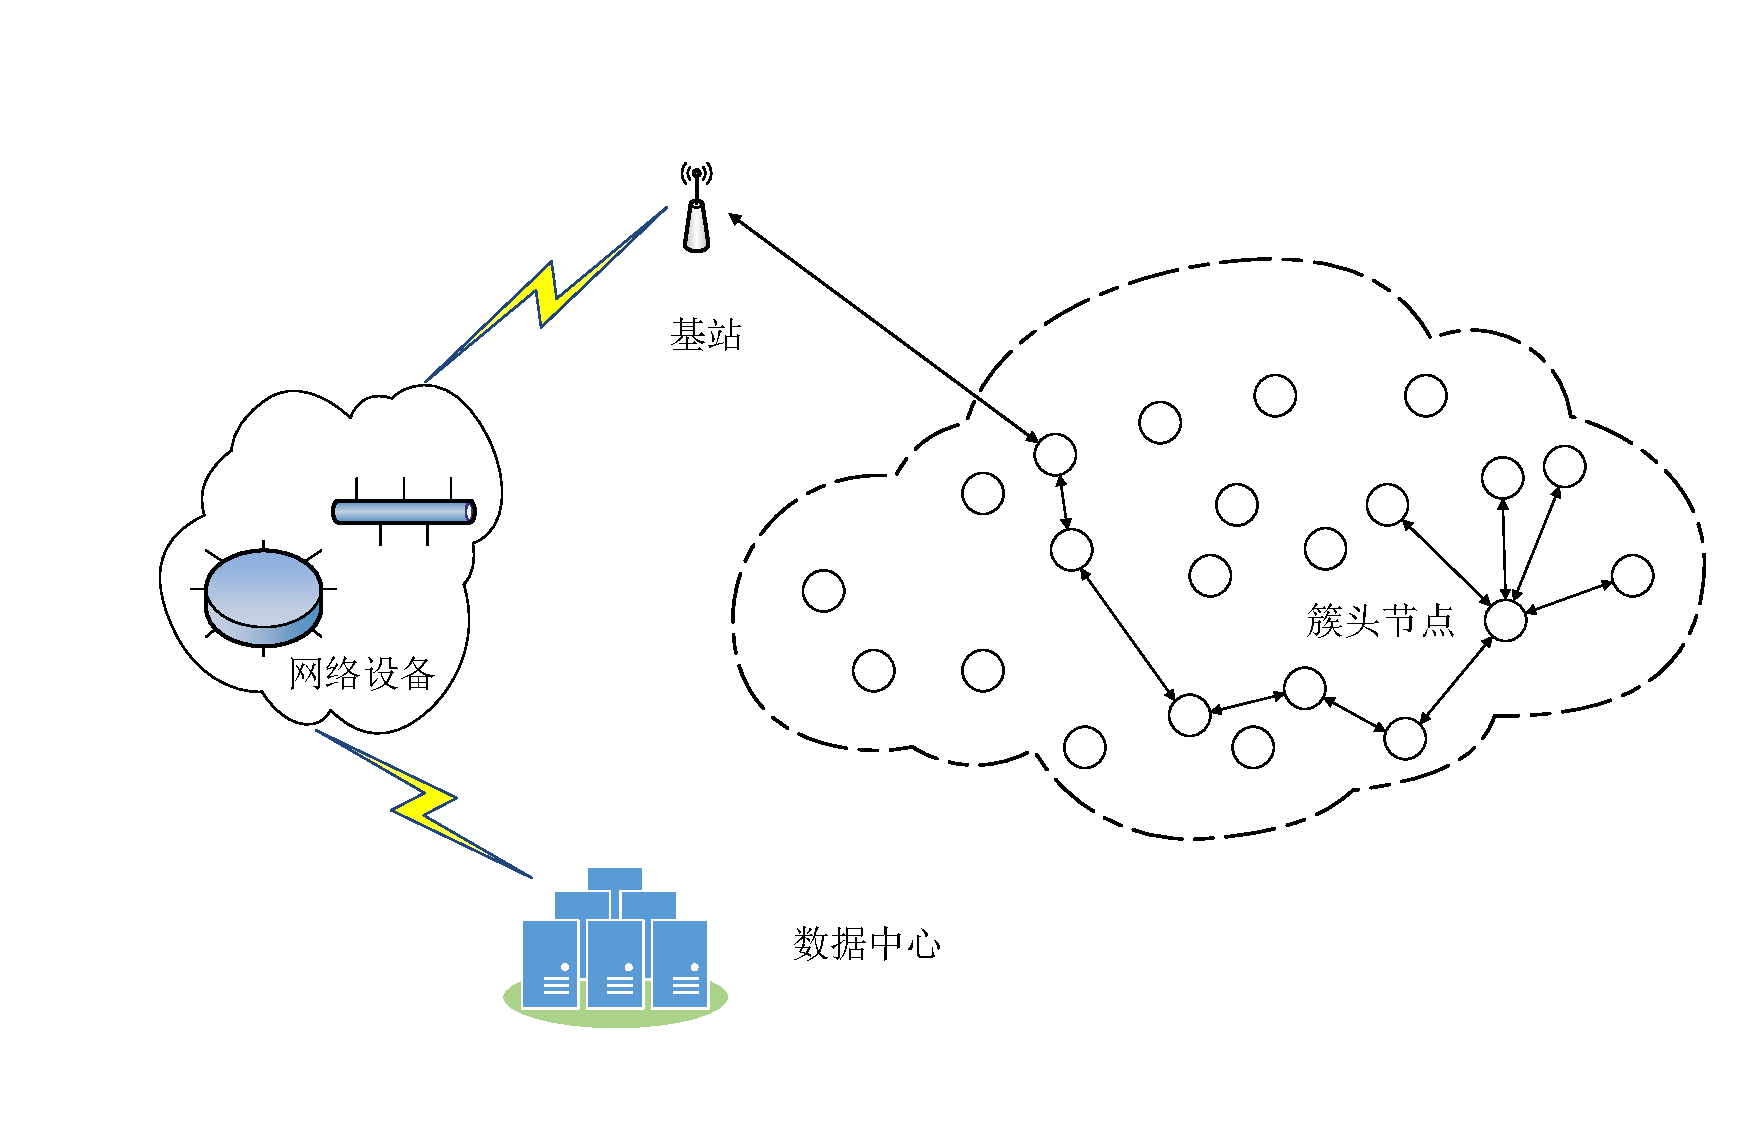
\includegraphics[width=5in]{cluster}
  \caption{无线传感网系统结构}
  \label{fig:cluster}
\end{figure}


无线传感网中,基站的计算和存储能力都比较强,
基站的功能可以是一个数据处理中心,向网络广播控制信息,从监测区域获取数据。
也可以是一个网络网关,负责数据向远程数据中心的传输。

\subsubsection{无线传感器节点结构}
传感器节点是无线传感网的基本组成单元,负责数据采集、发送等基本功能。
无线传感器节点一般仅具有很小的存储空间,较弱的计算能力,因此单个节点无法完成复杂的感知任务,需要大量的节点协同工作。

随着电子技术的发展,无线传感器节点的性能也有了很大的提升,如Crossbow公司研发的TelosB,CPU频率为8MHz,有10KB的RAM,使用2.4GHz无线电,能达到250Kbps数据传输,使用两节AAA电池(5号电池)供电。国产传感器节点典型的有美新的MEMSIC无线模块,工作频率可选433 MHz、868-915MHz或2.4GHz,拥有5年电池寿命,支持10-100米的发射范围,拥有19.2kbps-240kbps的数据传输速率。

\begin{figure}[htbp]
  \centering
  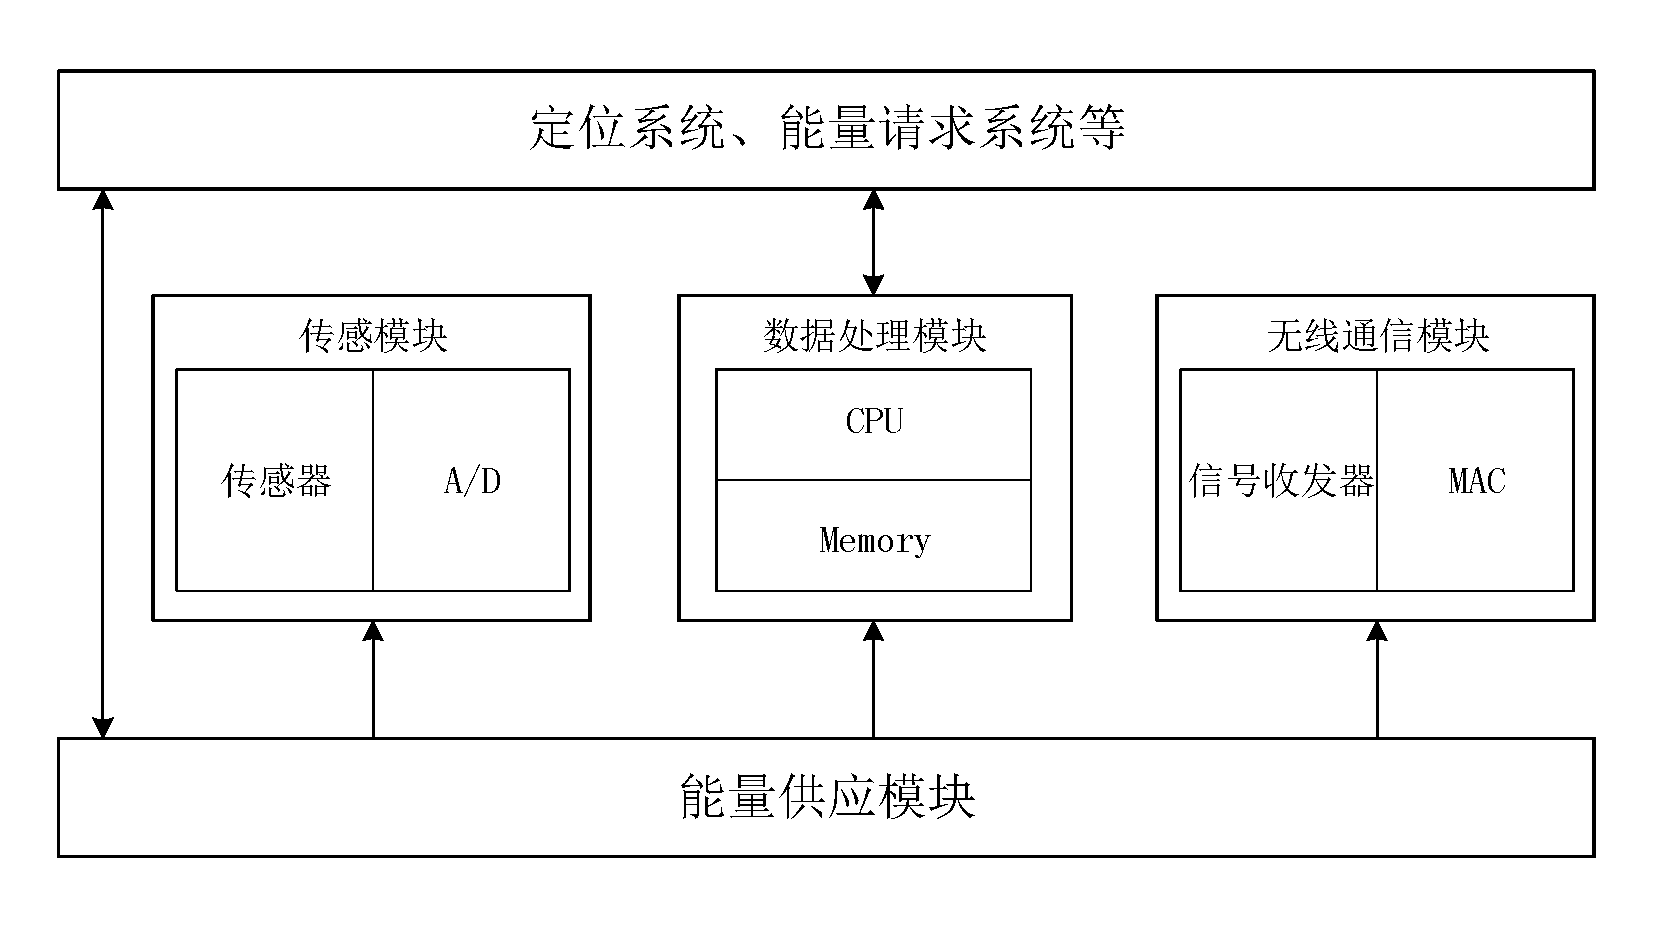
\includegraphics[width=5in]{node}
  \caption{无线传感网节点结构}
  \label{fig:node}
\end{figure}

这些传感器节点的设计原理基本相同,主要包括4个模块:传感模块、数据处理模块、无线通信模块和能量供应模块。
如图~\ref{fig:node}所示,是一个典型的无线传感器节点的结构图。传感模块主要负责从感知区域通过传感器获取数据,并将数据转化为适合进行网络传输的数字信号;数据处理模块主要包括处理和存储功能,负责控制传感器节点的运行,对传感模块获取的数据进行处理和存储,数据报文的整合与认证都是由数据处理模块完成,一般该模块需要嵌入式系统的支持,如UC Berkeley的开源嵌入式系统TinyOS\upcite{c:tinyos}等;无线通信模块负责与其他传感器节点或基站之间的通信,传感器节点一般使用内置天线进行数据收发;能量供应模块负责给其他模块供应能量,大部分传感器节点使用微型电池作为电源,因此能量非常有限。传感器节点中还包括一些负责定位、同步等功能的部件。

\subsubsection{无线传感网协议结构}

\begin{figure}[htbp]
  \centering
  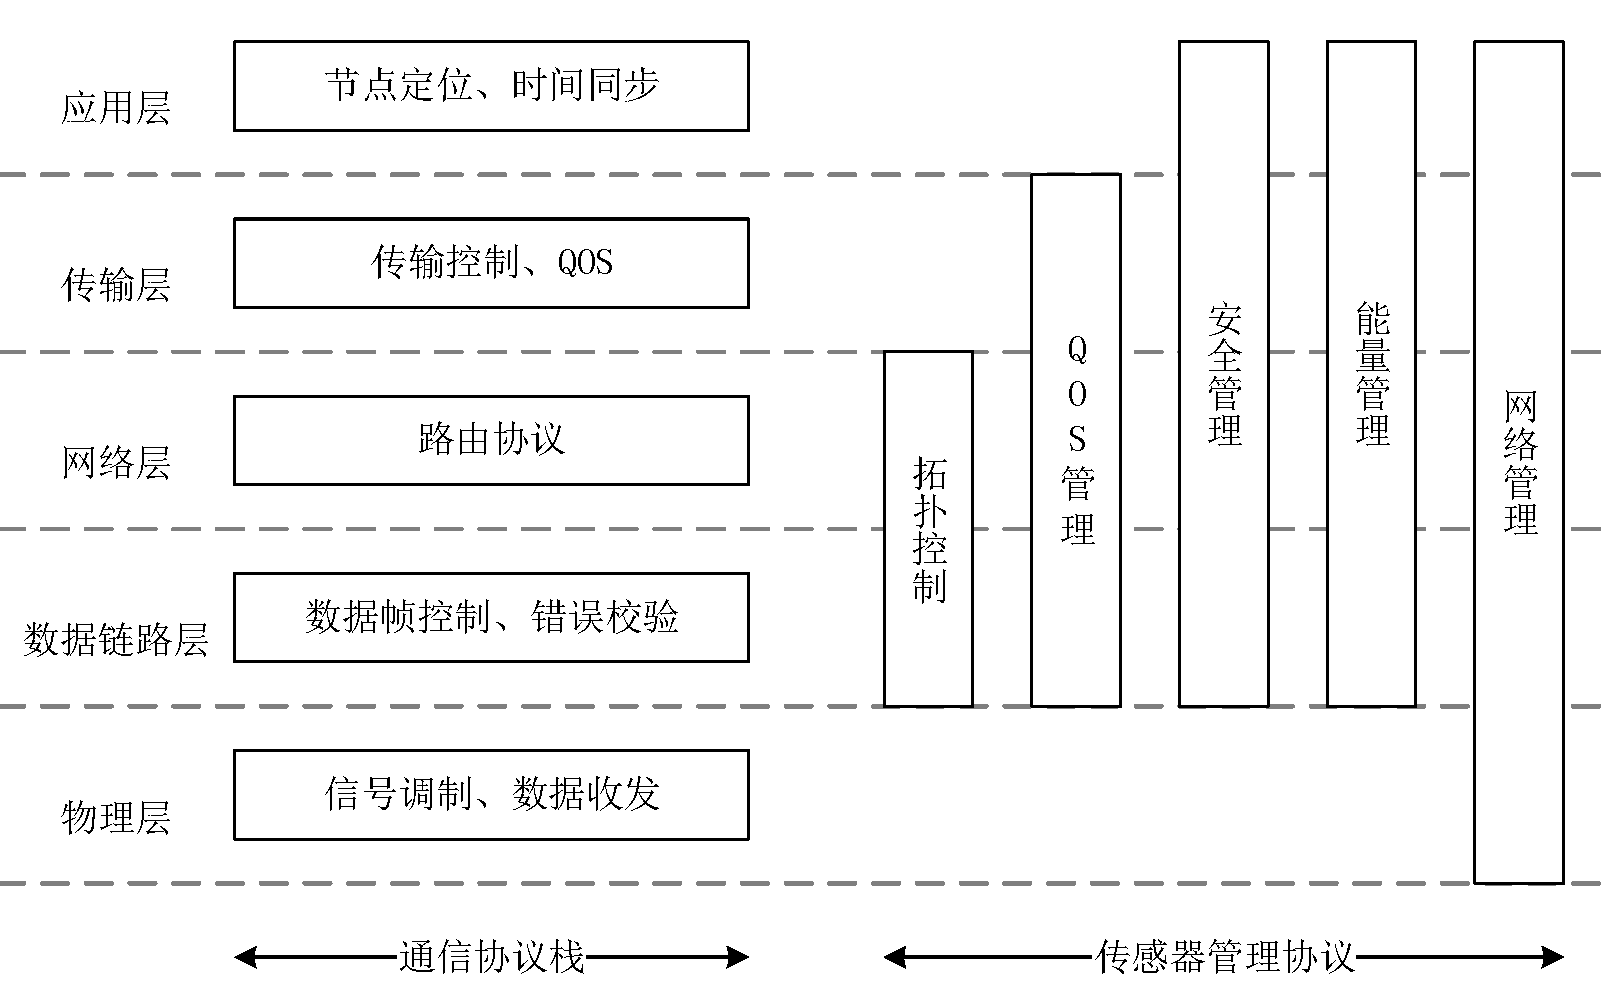
\includegraphics[width=5in]{construction}
  \caption{无线传感网协议结构}
  \label{fig:construction}
\end{figure}
无线传感网的通信协议栈和相关网络管理技术是当前的主要研究内容,协议结构如图~\ref{fig:construction}所示。
因为无线传感网是面向特定需求的网络,因此针对不同的部署环境,不同的网络部署结构,要对通信协议栈进行优化,使能量消耗、抗节点损耗、抗攻击能力等适应传感网的应用需求。

类似于OSI网络模型,无线传感网的通信协议栈由物理层、数据链路层、网络层、传输层、应用层组成:

物理层:物理层是通信协议栈的最底层,主要功能是将数据调制成适合传输的数字信号,通过无线电、红外灯无线介质完成传感器节点的数据收发。

数据链路层:数据链路层负责装配数据帧,对数据帧进行MAC校验,进行差错控制,向网络层提供透明可靠的数据传输服务。

网络层:主要负责无线传感网中的路由功能,将数据通过有效路径传送到目标节点,向传输层提供端对端的数据传输服务。

传输层:传输层负责数据报文的传送和控制,为应用层提供可靠的传输服务,对网络进行流量控制,进行服务质量控制(QOS)。

应用层:直接为应用提供服务,提供相应的应用协议和服务接口。

传感网管理协议提供了拓扑管理、QOS管理、安全管理、能量管理和网络管理等功能,实现对无线传感网以及各个节点的监控和管理。
\subsubsection{无线传感网的应用前景}
分布式传感网在军事中的应用是无线传感网的雏形,随着电子技术的不断发展,传感器节点的性能不断提升,无线传感网各种协议的完善和发展,使无线传感网在环境监测、军事侦察、智能家居、智能公路等各个领域得到了大量的应用,其应用前景十分广泛。

\begin{compactitem}
  \item 环境监测:无线传感网能完成大范围监测的任务,在自然数据采集中发挥重要作用,尤其是海洋监测传感网和内陆水文传感网等应用领域。如Li 等人将无线传感网部署在水产养殖水域,对水环境数据进行检测\upcite{c:water}。
  \item 军事侦察:由于无线传感网具有自组网、部署简单、容许节点失效等特点,适合部署在危险的敌对区域,完成军事侦察、战场环境监测等任务,因而在军事领域有很大应用前景,是现代化电子战的重要战略武器。如美国海军将开发的自主分布式DADS(Deployable Autonomous Distributed System)用于沿海广大海域的警戒、反潜和反水雷\upcite{c:DADS}。
  \item 智能家居:智能家居是通过无线传感器将房间中的各种家电等设备连接起来,实现家居环境的监测以及远程控制,构建出智能的居住环境\upcite{c:homes}。
  \item 智能公路:通过部署在公路上的无线传感器节点以及车载传感器节点,共同组成智能公路传感网络,对交通状况实现自动监测,引导车流等,实现自动化的公路交通管理。
\end{compactitem}



\subsection{规模化无线传感网数据认证}
\subsubsection{规模化无线传感网的特点}
规模化无线传感网是为满足大范围监测的需要而产生的,如国内著名的绿野千传项目,在浙江省天目山建立的大规林业监测传感网,部署的自组织传感网节点超过2000个,网络中传输路径跳数超过 20 跳
\upcite{c:lvye}。
规模化无线传感网具有如下的特点:
\begin{enumerate}\setlength{\itemsep}{-\itemsep}
  \item 节点数量大,覆盖面积广,节点失效较为频繁,网络拓扑结构相对不稳定。
  \item 一般部署于恶劣区域,甚至是敌对攻击区域,恶意攻击的频度增加。
  \item 节点的计算和存储能力更为受限,网络的能量较为敏感,对机制的轻量化要求更突出。
\end{enumerate}

\subsubsection{规模化无线传感网的数据认证需求}
无线传感网中的认证包括身份认证和数据认证。身份认证是对网络中节点的合法身份的一种判定机制,是数据认证的基础。无线传感网数据认证主要包括两个方面:
\begin{compactitem}
  \item 数据来源合法性,主要以身份认证为基础,通过数据报文中的认证机制判定数据报文的来源的合法性。
  \item 数据完整性,通过数据认证的机制,确保节点收到的数据报文没有被非法进行篡改。
\end{compactitem}

在环境监测等领域,规模化传感网每天都会产生海量的感知数据。在军事侦察领域,随着侦察区域的扩大,侦察精度的提高,传感网感知的数据量飞速增长。尤其在实时监测场景,数据量大、传输实时性要求高,无线传感器节点的性能限制使得规模化传感网实现可靠传输具有非常的难度,合适的数据认证机制可以为其提供有力支持。在无线传感网中数据泄露、错误数据甚至虚假数据会对网络的安全造成重大影响。尤其在重要战略场景或军事场景,还要考虑破坏攻击的可能,因此数据认证更为安全攸关。
\subsubsection{规模化无线传感网数据认证面临的挑战}

复杂环境下数据高安全性要求对数据认证提出的挑战。实时监测传感网通常部署环境恶劣,而且缺乏基础设施的建设,由于自然环境和主动攻击等对节点的破坏,使节点的失效率很高,网络拓扑结构动态变化,数据传输质量不够稳定,而且存在突发大故障潜因,需要在容灾抗毁前提下进行数据认证,确保传输的安全性。

端对端传输为数据认证提出的挑战。完全依靠广播等数据传输机制,在规模化无线传感网中,传输效率过低,消耗的节点能量和通信资源过大,而且容易受到泛洪攻击的影响。有效利用规模化传感网中端对端数据传输,能够有效的保证传输效率。在端对端传输中,由于多跳传输的原因,当路径中出现妥协节点时,整条路径容易被攻破,从而造成数据传输被攻击,因而在多路径端对端的数据传输中,有效利用数据认证机制加强路径上的安全保障是安全传输的关键。

轻量级认证机制及其实现技术为数据认证提出的挑战。规模化无线传感网传输的数据量大,要求处理快捷。在节点资源能力受限,通信能耗受限的前提下,需要计算、存储、通信都轻量级的水平,保障网络安全、传输可靠性、高效性和数据可信,具有很大难度。传统的的认证机制使用的密码算法复杂度未达到轻量级,不适合规模化传感网网络资源受限的特点,我们需要设计适合实时性较高的规模无线传感网达到轻量级算法。

攻击对抗对数据认证提出的挑战。无线传感网一般部署在恶劣环境中,而且具有自组网络的多跳性、无中心性和自组织性等特征,致使其通信协议栈的各个层级都容易遭受到各种形式的攻击,我们需要设计能够适应有限节点能量,有限计算能力的数据认证算法,对抗各种攻击,保证无线传感网传输数据的来源合法性和完整性。

\section{本文研究内容}
本文根据规模化无线传感网的安全需求以及其特点,针对其数据认证关键技术展开研究,使用多节点联合的技术思路研究数据认证模型和机制,并设计实现了关键算法。
主要工作如下:

\begin{enumerate}\setlength{\itemsep}{-\itemsep}
  \item 提出了多跳长路径上多节点联合数据认证的模型,设计了多跳长路径上多节点联合数据认证协议,并设计了路径上节点关系的维护算法,对协议的安全性能进行了分析评价。
  \item 针对多跳长路径上多写点联合数据认证协议的不足,对算法进行了优化,提出了多路径抗节点失效机制和动态步长多节点联合数据认证机制,并对优化方案的安全性能进行了分析评价。
  \item 围绕多跳长路径多节点联合数据认证机制的需求,对密钥分配方案进行了深入研究,提出了基于单向hash链的密钥分配方案,并对认证中的MAC进行了研究,提出了适应数据认证机制需求的MAC码。
\end{enumerate}


\section{本文组织结构}
本文一共分为七章。

第一章\quad 绪论,介绍了课题的选题背景,描述了无线传感网的特点,介绍了无线传感网的相关安全技术,列出了本文的主要研究内容和本文组织结构。

第二章\quad 相关研究概述,本章首先对无线传感网的安全技术进行了概述,然后重点对数据认证和密钥分配两种安全技术进行了论述。

第三章\quad 多跳长路径上多节点联合数据认证,本章提出了无线传感网中多跳长路径多节点联合的数据认证模型,及其设计目标。
重点介绍了关键算法与协议的设计实现,对多节点联合数据认证机制的安全性能进行了分析评价。

第四章\quad 数据认证方案优化,本章针对多跳长路径上多节点联合数据认证进行了优化,提出了多路径抗节点失效和动态步长多节点联合数据认证两个优化方案,并对它们的安全性能进行了分析评价。

第五章\quad 密钥分配与MAC设计,本章对多节点联合数据认证中的密钥分配方案以及使用的MAC的设计进行了介绍,提出了基于单向hash链的密钥分配方案,以及适应多节点联合数据认证的MAC码。

第六章\quad 仿真实验与结果分析,本章在仿真平台上对多跳长路径多节点联合数据认证机制,以及其优化方案进行了仿真实验,对它们的安全性能结果进行了评价。

第七章\quad 总结与展望,本章对全文的工作做了总结,指出了数据认证机制现阶段的不足以及未来研究中需要研究及完善的地方。


% \chapter{中华人民共和国}
\label{cha:china}

\section{图的例子}
\label{sec:other}

在第~\ref{cha:intro} 章中我们学习了贝叶斯公式~(\ref{equ:chap1:bayes}),这里我们复
习一下:
\begin{equation}
\label{equ:chap2:bayes}
p(y|\mathbf{x}) = \frac{p(\mathbf{x},y)}{p(\mathbf{x})}=
\frac{p(\mathbf{x}|y)p(y)}{p(\mathbf{x})}
\end{equation}

\subsection{绘图}
\label{sec:draw}

本模板不再预先装载任何绘图包(如 \textsf{pstricks,pgf} 等),完全由你自己来决定。
个人觉得 \textsf{pgf} 不错,不依赖于 Postscript。此外还有很多针对 \LaTeX{} 的
 GUI 作图工具,如 XFig(jFig), WinFig, Tpx, Ipe, Dia, Inkscape, LaTeXPiX,
jPicEdt, jaxdraw 等等。

\subsection{插图}
\label{sec:graphs}
关于子图形的使用细节请参看 \textsf{subcaption} 的说明文档。

\subsection{一个图形}
\label{sec:onefig}
一般图形都是处在浮动环境中。之所以称为浮动是指最终排版效果图形的位置不一定与源文
件中的位置对应\footnote{This is not a bug, but a feature of
\LaTeX!},这也是刚使 用 \LaTeX{}
同学可能遇到的问题。如果要强制固定浮动图形的位置,请使用
\textsf{float} 宏包, 它提供了 \texttt{[H]}
参数,比如图~\ref{fig:heythere}。
\begin{figure}[H] % use float package if you want it here
  \centering
  
\includegraphics[height=2cm]{hello.jpg}
  \caption{插个图插个图}
  \label{fig:heythere}
\end{figure}

大学之道,在明明德,在亲民,在止于至善。知止而后有定;定而后能静;静而后能安;安
而后能虑;虑而后能得。物有本末,事有终始。知所先后,则近道矣。古之欲明明德于天
下者,先治其国;欲治其国者,先齐其家;欲齐其家者,先修其身;欲修其身者,先正其心;
欲正其心者,先诚其意;欲诚其意者,先致其知;致知在格物。物格而后知至;知至而后
意诚;意诚而后心正;心正而后身 修;身修而后家齐;家齐而后国治;国治而后天下
平。自天子以至于庶人,壹是皆以修身为本。其本乱而未治者 否矣。其所厚者薄,而其所
薄者厚,未之有也!

\hfill \pozhehao《大学》


\subsection{简单子图}
\label{sec:multifig}

如果多个图形相互独立,并不共用一个图形计数器,那么用 \verb|minipage| 或者
\verb|parbox| 就可以。否则,请参看图~\ref{fig:big1},它包含两个小图,分别是图~\ref{fig:subfig1}
和图~\ref{fig:subfig2}。推荐使用 \verb|\subcaption|,不要再用\verb|\subfloat|,\verb|\subfigure| 和 \verb|\subtable|了。
\begin{figure} %[h]
  \centering%
  \subcaptionbox{第一个小图形\label{fig:subfig1}}{%    
    
\includegraphics[height=2cm]{tongji-fig-logo.png}}\hspace{4em}%
  \subcaptionbox{第二个小图形。如果标题很长的话,它会自动换行,这个 caption 就是这样的例子\label{fig:subfig2}}{%    
    
\includegraphics[height=2cm]{tongji-text-logo.png}}
  \caption{包含子图形的大图形}
  \label{fig:big1}
\end{figure}

古之学者必有师。师者,所以传道受业解惑也。人非生而知之者,孰能无惑?惑而不从师,
其为惑也,终不解矣。生乎吾前,其闻道也固先乎吾,吾从而师之;生乎吾後,其闻道也亦
先乎吾,吾从而师之。吾师道也,夫庸知其年之先後生於吾乎!是故无贵无贱无长无少,道
之所存,师之所存也。

嗟乎!师道之不传也久矣,欲人之无惑也难矣。古之圣人,其出人也远矣,犹且从师而问焉;
今之众人,其下圣人也亦远矣,而耻学於师。是故圣益圣,愚益愚。圣人之所以为圣,愚
人之所以为愚,其皆出於此乎?爱其子,择师而教之,於其身也,则耻师焉,惑焉。彼童子
之师,授之书而习其句读者,非吾所谓传其道、解其惑者也。句读之不知,惑之不解,或师
焉,或不焉,小学而大遗,吾未见其明也。巫医、乐师、百工之人不耻相师,  士大夫之族
曰“师”曰“弟子”之云者,则群聚而笑之。问之,则曰:彼与彼年相若也,道相似也,位
卑则足羞,官盛则近谀。呜呼!师道之不复,可知矣。巫医、乐师、百工之人。吾子不齿,
今其智乃反不能及,其可怪也欤!圣人无常师。孔子师郯子、苌子、师襄、老聃。郯子之徒,
其贤不及孔子。孔子曰:“三人行,必有我师。”是故弟子不必不如师,师不必贤於弟子。
闻道有先後,术业有专攻,如是而已。

\subsection{复杂子图要注意遮挡}
使用子图的方法如图~\ref{fig:chap2:zitu}所示,使用\texttt{subcaptionbox}环境设置每一个子图,注意\texttt{subcaptionbox}其后需要有括号,以及子图换行时需要使用\texttt{vskip},以免下一排子图会对上一排子图的图名造成遮挡。
\begin{figure}[htbp]
\centering
  \subcaptionbox{第一个小图形}{\label{fig:chap1:zitu:a}
  
\includegraphics[width=5cm]{tongji-fig-logo}\hskip2cm}
  \subcaptionbox{第二个小图形}{\label{fig:chap1:zitu:b}
  
\includegraphics[width=5cm]{tongji-fig-logo}}
\vskip0.5cm
  \subcaptionbox{第三个小图形}{\label{fig:chap1:zitu:c}
  
\includegraphics[width=5cm]{tongji-fig-logo}\hskip2cm}
  \subcaptionbox{第四个小图形}{\label{fig:chap1:zitu:d}
  
\includegraphics[width=5cm]{tongji-fig-logo}}
\caption{多子图用\texttt{subcaptionbox}}\label{fig:chap2:zitu}
\end{figure}


\subsection{多个图形独立}
如果要把编号的两个图形并排,那么小页就非常有用了,如图~\ref{fig:parallel2}:
\begin{figure}
\begin{minipage}{0.48\textwidth}
  \centering
  
\includegraphics[height=2cm]{tongji-whole-logo.png}
  \caption{并排第一个图}
  \label{fig:parallel1}
\end{minipage}\hfill
\begin{minipage}{0.48\textwidth}
  \centering
  
\includegraphics[height=2cm]{tongji-whole-logo.png}
  \caption{并排第二个图}
  \label{fig:parallel2}
\end{minipage}
\end{figure}


李氏子蟠,年十七,好古文、六艺,经传皆通习之,不拘於时,学於余。余嘉其能行古
道,作师说以贻之。

\hfill \pozhehao 韩愈(唐)


\subsection{插图大原则}
同志们,如果遇到问题一定要会搜索,要么看别人的问答,要么看宏包的文档,希望你不要成为重度伸手党。
一点微小的工作,谢谢大家。

\section{插入pdf格式图片的问题}
\label{sec:problem}
在\LaTeX{}中插入高清图片一般有两种方式:1)插入~eps~矢量图,2)插入~pdf~格式图片。在模板测试过程中遇到一个插入
~pdf~格式图片的问题。

问题描述

插入~pdf~格式的图,有时采用~XeLaTeX~编译后,插图被翻转~90~度。有时却不会出现该问题。问题图片如图~\ref{rotatedBode}~所示。
\begin{figure}[H] 
  \centering
  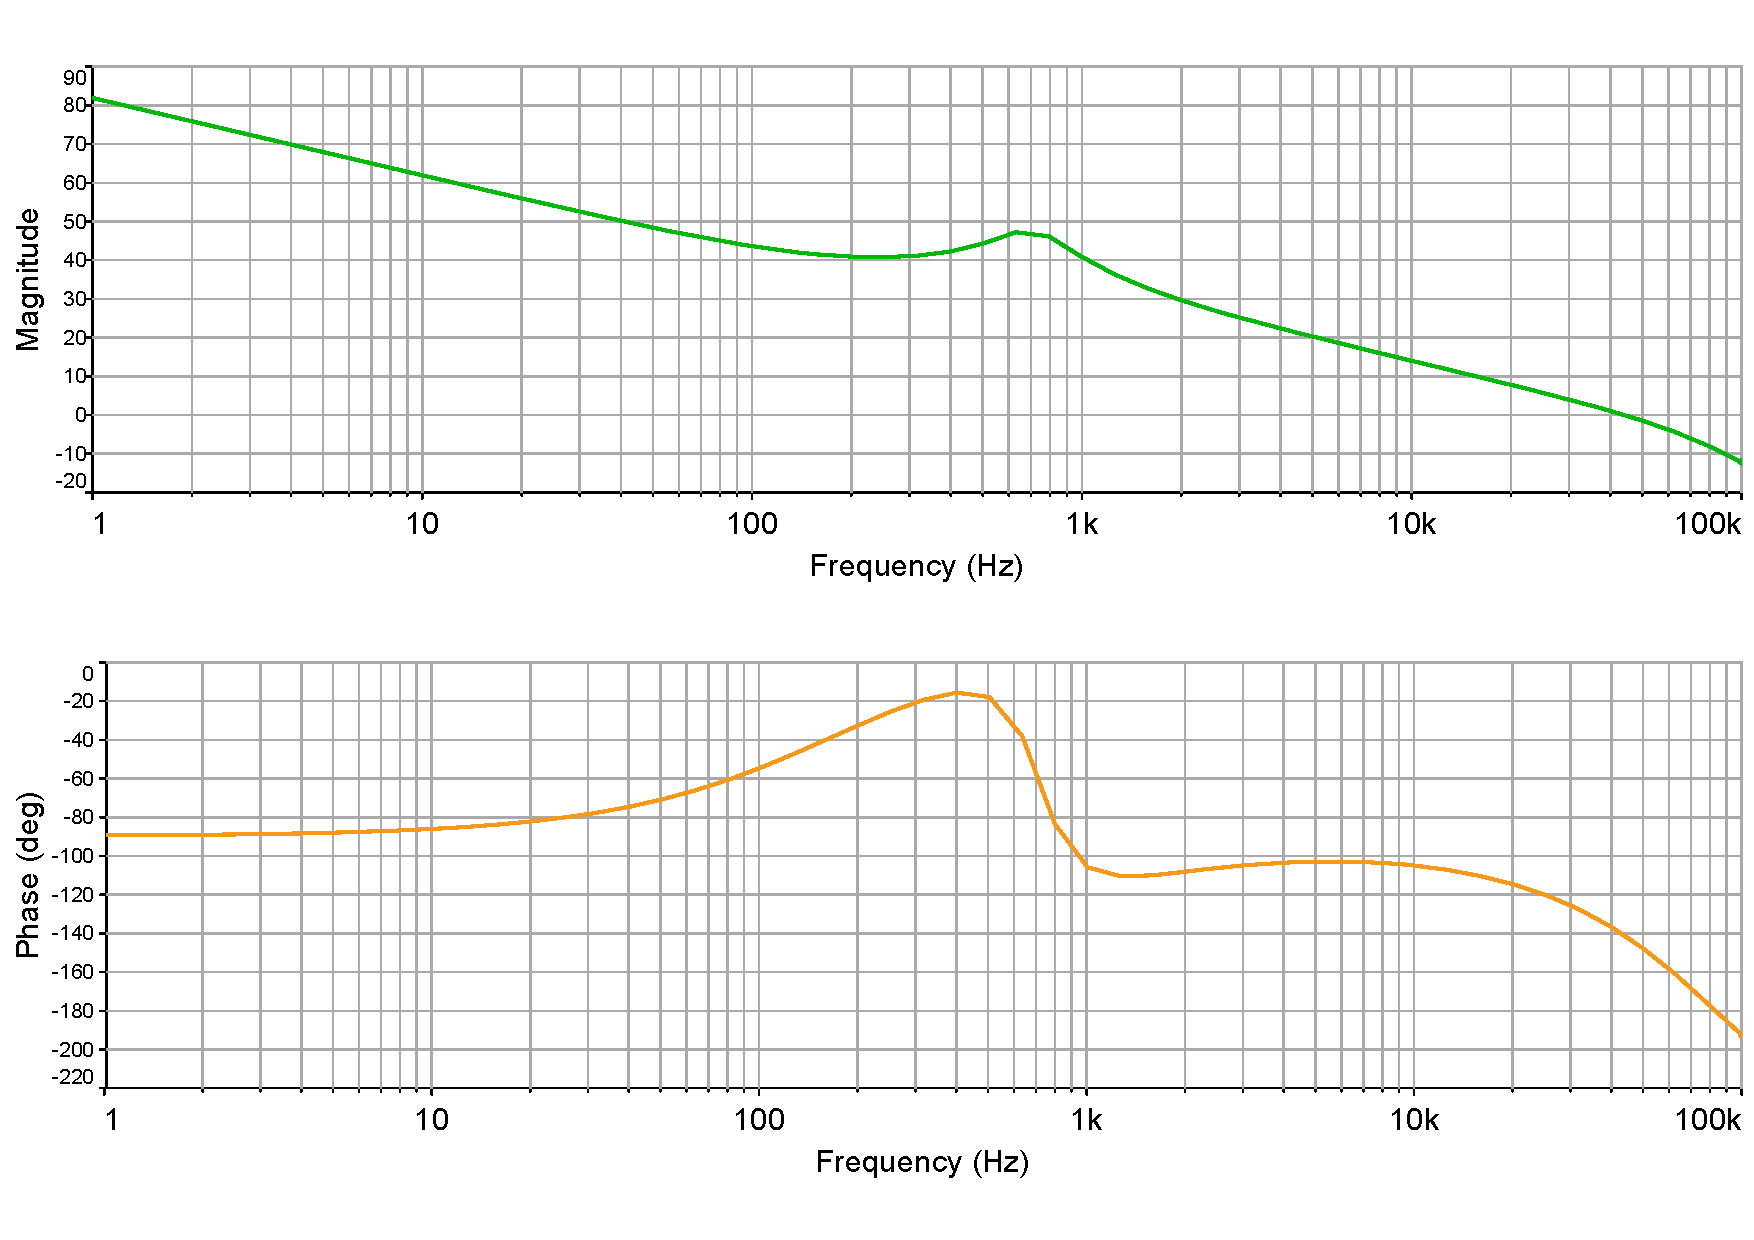
\includegraphics[width=12cm]{BodeGraph.pdf}
  \caption{被自动翻转的bode图}
  \label{rotatedBode}
\end{figure}

问题原因

同一幅图片,XeLaTeX~编译出现图片翻转,而~pdfLaTeX~编译,输出正常。
原因可能是出现在~XeLaTeX~编译过程中会将有些~pdf~文件自身多余的旋转命令编译出来。

问题解决方法

第一种方法(抄自刘海洋大牛的方案):
使用命令\\ \texttt{pdfcrop foo.pdf foo-new.pdf},当然,新文件名可以和旧文件名相同。 这个方法的好处就是 pdfcrop 是texlive自带的,我装的是texlive2017,因此自带了。

第二种方法:采用GhostScript软件消除多余的旋转命令。
\begin{enumerate}
    \item 下载安装~GhostScript~软件,官网为\url{https://www.ghostscript.com/download/gsdnld.html/}
        
    \item 将安装后的bin文件夹地址加入用户环境变量,在我电脑上为~\verb|D:|\verb|\Program Files|\verb|\gs|\verb|\gs9.22|\verb|\bin|
	
    \item cmd~命令行进入想转换图片所在文件夹,执行命令\\gswin32c -sDEVICE=pdfwrite -o newname.pdf  previousname.pdf
              得到一个去除多余旋转命令的~newname.pdf~文件。

    \item 在\LaTeX{}中插入该~pdf~文件,XeLaTeX~编译。
\end{enumerate}

处理之后的图片如图~\ref{Bode}~所示。
\begin{figure}[H] 
  \centering
  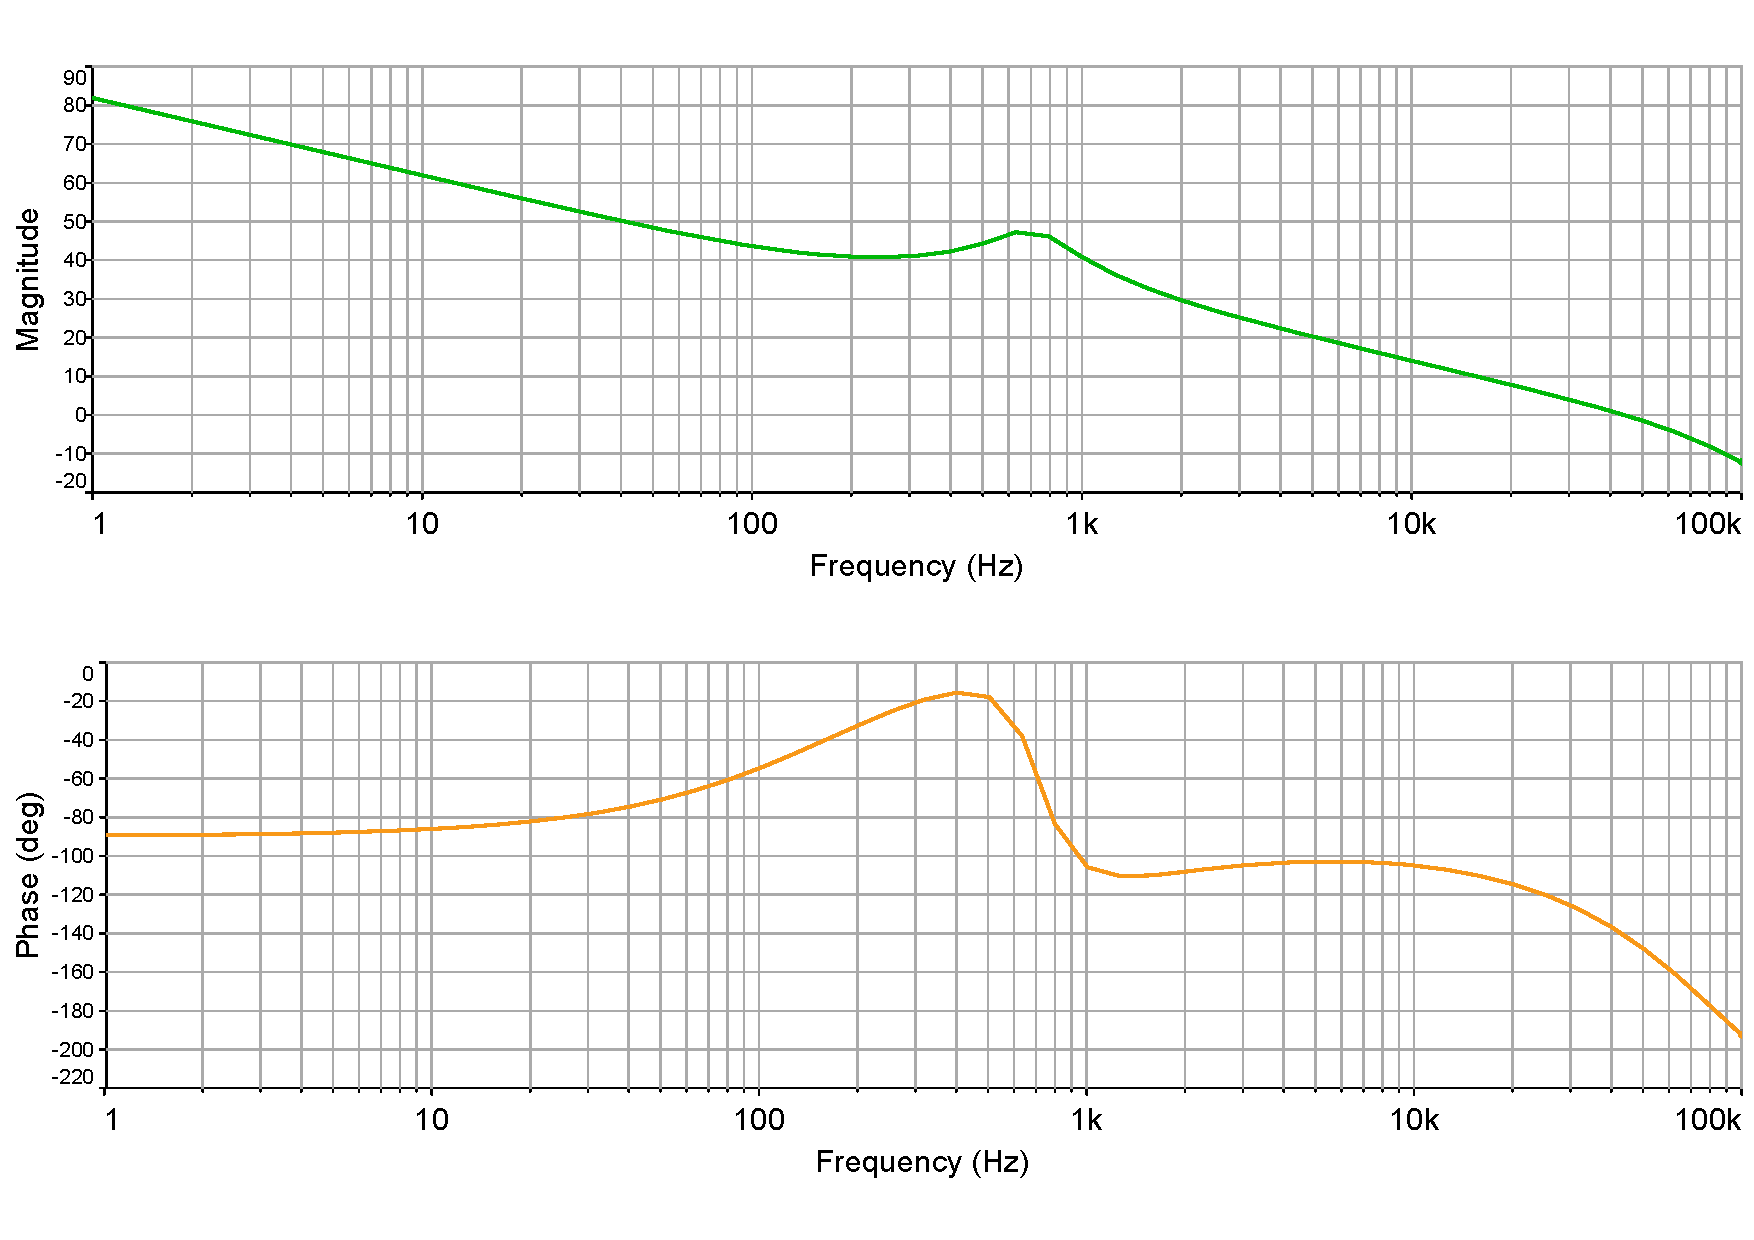
\includegraphics[width=12cm]{Bode.pdf}
  \caption{处理后的bode图}
  \label{Bode}
\end{figure}






% \include{parts/examples/digitalexp}
% \begin{frame}[fragile]
	\frametitle{An Algorithm For Finding Prime Numbers.}
	%使用空格进行缩进
	\begin{lstlisting}[language=python,xleftmargin=-4em,xrightmargin=2em, aboveskip=1em,framexleftmargin = -4em,framexrightmargin = 4em]
	def getRankingDistribution(self, lambda_setting):
	
	    p = []
	    p.append(npy.exp(-1.0 / lambda_setting))
	    
	    for k in range(1, self.node_num):
	        temp = -1.0 * (k + 1) / lambda_setting
	        p.append(npy.exp(temp) + p[k - 1])
	        
	    return p;
	\end{lstlisting}
	
\end{frame}

\begin{frame}[fragile]
	
	\begin{lstlisting}[language=python,xleftmargin=-4em,xrightmargin=2em, aboveskip=1em,framexleftmargin = -4em,framexrightmargin = 4em]
	def getCate(self, u_vec, v_vec):
	    p = []
	    p.append(u_vec[0] * v_vec[0])
	    
	    for k in range(1, self.Z):
	        p.append(p[k - 1] + u_vec[k] * v_vec[k])
	    
	    q = npy.random.uniform() * p[self.Z - 1]
	    for f in range(self.Z):
	        if(p[f] > q):
	            break
	            
	    return f;
	\end{lstlisting}
\end{frame}


\begin{frame}[fragile]
%	\scalebox{0.8}{
%		\parbox{1.2\textwidth}{
			\begin{lstlisting}[language=python,xleftmargin=-15em,xrightmargin=2em, aboveskip=0.2em,framexleftmargin = -14em,framexrightmargin = 4em]
			def draw_CA_BPR(self, uL, vL,
			           u_cat_vars, v_cat_vars, item_sorts):
			    res = []
			    for u in self.graph:
			        for v in self.graph[u]:
			        cate = self.getCate(uNorm[self.user_set[u]], 
			                    vNorm[self.item_set[v]])
			        self.cate_count[cate] += 1
			        while 1 :
			            r = self.getPos(self.vSum)
			            if(uL[self.user_set[u], cate] < 0):
			                r = self.vSum - r - 1
			            vj = self.node_set[item_sorts[cate][r]] 
			            if(self.graph[u].has_key(vj) == False):
			                break
			         res.append((u, v, vj))
			    random.shuffle(res)
			    return res;
			\end{lstlisting}
	%	}
	%}
	
\end{frame}

%\end{frame} can NOT be indented
%\end{frame} cannot have any comments directly after it
%\end{frame}不能缩进
% \backmatter
% \listoffigures
% \listoftables
% \listofequations
% \bibliographystyle{ref/numeric} % ref/numeric,ref/author-year,plainnat,IEEEtran
% \bibliography{ref/refs}
% %%% Local Variables:
%%% mode: latex
%%% TeX-master: "../main"
%%% End:

\begin{ack}
  衷心感谢导师 xxx 教授和物理系 xxx 副教授对本人的精心指导。他们的言传身教将使
  我终生受益。

  在美国麻省理工学院化学系进行九个月的合作研究期间,承蒙 xxx 教授热心指导与帮助,不
  胜感激。感谢 xx 实验室主任 xx 教授,以及实验室全体老师和同学们的热情帮助和支
  持!本课题承蒙国家自然科学基金资助,特此致谢。

  感谢 \ucasthesis,它的存在让我的论文写作轻松自在了许多,让我的论文格式规整漂亮了
  许多。
\end{ack}

% \begin{appendix}
%   \chapter{外文资料原文}
\label{cha:engorg}

\title{The title of the English paper}

\textbf{Abstract:} As one of the most widely used techniques in operations
research, \emph{ mathematical programming} is defined as a means of maximizing a
quantity known as \emph{bjective function}, subject to a set of constraints
represented by equations and inequalities. Some known subtopics of mathematical
programming are linear programming, nonlinear programming, multiobjective
programming, goal programming, dynamic programming, and multilevel
programming$^{[1]}$.

It is impossible to cover in a single chapter every concept of mathematical
programming. This chapter introduces only the basic concepts and techniques of
mathematical programming such that readers gain an understanding of them
throughout the book$^{[2,3]}$.


\section{Single-Objective Programming}
The general form of single-objective programming (SOP) is written
as follows,
\begin{equation*} % 如果附录中的公式不想让它出现在公式索引中,那就请
                             % 用 equation*
\left\{\begin{array}{l}
\max \,\,f(x)\\[0.1 cm]
\mbox{subject to:} \\ [0.1 cm]
\qquad g_j(x)\le 0,\quad j=1,2,\cdots,p
\end{array}\right.
\end{equation*}
which maximizes a real-valued function $f$ of
$x=(x_1,x_2,\cdots,x_n)$ subject to a set of constraints.

\newcommand\Real{\mathbf{R}}
\newtheorem{mpdef}{Definition}[chapter]
\begin{mpdef}
In SOP, we call $x$ a decision vector, and
$x_1,x_2,\cdots,x_n$ decision variables. The function
$f$ is called the objective function. The set
\begin{equation*}
S=\left\{x\in\Real^n\bigm|g_j(x)\le 0,\,j=1,2,\cdots,p\right\}
\end{equation*}
is called the feasible set. An element $x$ in $S$ is called a
feasible solution.
\end{mpdef}

\newtheorem{mpdefop}[mpdef]{Definition}
\begin{mpdefop}
A feasible solution $x^*$ is called the optimal
solution of SOP if and only if
\begin{equation}
f(x^*)\ge f(x)
\end{equation}
for any feasible solution $x$.
\end{mpdefop}

One of the outstanding contributions to mathematical programming was known as
the Kuhn-Tucker conditions\ref{eq:ktc}. In order to introduce them, let us give
some definitions. An inequality constraint $g_j(x)\le 0$ is said to be active at
a point $x^*$ if $g_j(x^*)=0$. A point $x^*$ satisfying $g_j(x^*)\le 0$ is said
to be regular if the gradient vectors $\nabla g_j(x)$ of all active constraints
are linearly independent.

Let $x^*$ be a regular point of the constraints of SOP and assume that all the
functions $f(x)$ and $g_j(x),j=1,2,\cdots,p$ are differentiable. If $x^*$ is a
local optimal solution, then there exist Lagrange multipliers
$\lambda_j,j=1,2,\cdots,p$ such that the following Kuhn-Tucker conditions hold,
\begin{equation}
\label{eq:ktc}
\left\{\begin{array}{l}
    \nabla f(x^*)-\sum\limits_{j=1}^p\lambda_j\nabla g_j(x^*)=0\\[0.3cm]
    \lambda_jg_j(x^*)=0,\quad j=1,2,\cdots,p\\[0.2cm]
    \lambda_j\ge 0,\quad j=1,2,\cdots,p.
\end{array}\right.
\end{equation}
If all the functions $f(x)$ and $g_j(x),j=1,2,\cdots,p$ are convex and
differentiable, and the point $x^*$ satisfies the Kuhn-Tucker conditions
(\ref{eq:ktc}), then it has been proved that the point $x^*$ is a global optimal
solution of SOP.

\subsection{Linear Programming}
\label{sec:lp}

If the functions $f(x),g_j(x),j=1,2,\cdots,p$ are all linear, then SOP is called
a {\em linear programming}.

The feasible set of linear is always convex. A point $x$ is called an extreme
point of convex set $S$ if $x\in S$ and $x$ cannot be expressed as a convex
combination of two points in $S$. It has been shown that the optimal solution to
linear programming corresponds to an extreme point of its feasible set provided
that the feasible set $S$ is bounded. This fact is the basis of the {\em simplex
  algorithm} which was developed by Dantzig as a very efficient method for
solving linear programming.
\begin{table}[ht]
\centering
  \centering
  \caption*{Table~1\hskip1em This is an example for manually numbered table, which
    would not appear in the list of tables}
  \label{tab:badtabular2}
  \begin{tabular}[c]{|m{1.5cm}|c|c|c|c|c|c|}\hline
    \multicolumn{2}{|c|}{Network Topology} & \# of nodes &
    \multicolumn{3}{c|}{\# of clients} & Server \\\hline
    GT-ITM & Waxman Transit-Stub & 600 &
    \multirow{2}{2em}{2\%}&
    \multirow{2}{2em}{10\%}&
    \multirow{2}{2em}{50\%}&
    \multirow{2}{1.2in}{Max. Connectivity}\\\cline{1-3}
    \multicolumn{2}{|c|}{Inet-2.1} & 6000 & & & &\\\hline
    \multirow{2}{1.5cm}{Xue} & Rui  & Ni &\multicolumn{4}{c|}{\multirow{2}*{\thuthesis}}\\\cline{2-3}
    & \multicolumn{2}{c|}{ABCDEF} &\multicolumn{4}{c|}{} \\\hline
\end{tabular}
\end{table}

Roughly speaking, the simplex algorithm examines only the extreme points of the
feasible set, rather than all feasible points. At first, the simplex algorithm
selects an extreme point as the initial point. The successive extreme point is
selected so as to improve the objective function value. The procedure is
repeated until no improvement in objective function value can be made. The last
extreme point is the optimal solution.

\subsection{Nonlinear Programming}

If at least one of the functions $f(x),g_j(x),j=1,2,\cdots,p$ is nonlinear, then
SOP is called a {\em nonlinear programming}.

A large number of classical optimization methods have been developed to treat
special-structural nonlinear programming based on the mathematical theory
concerned with analyzing the structure of problems.
\begin{figure}[h]
  \centering
  
\includegraphics{thu-lib-logo.pdf}
  \caption*{Figure~1\quad This is an example for manually numbered figure,
    which would not appear in the list of figures}
  \label{tab:badfigure2}
\end{figure}

Now we consider a nonlinear programming which is confronted solely with
maximizing a real-valued function with domain $\Real^n$.  Whether derivatives are
available or not, the usual strategy is first to select a point in $\Real^n$ which
is thought to be the most likely place where the maximum exists. If there is no
information available on which to base such a selection, a point is chosen at
random. From this first point an attempt is made to construct a sequence of
points, each of which yields an improved objective function value over its
predecessor. The next point to be added to the sequence is chosen by analyzing
the behavior of the function at the previous points. This construction continues
until some termination criterion is met. Methods based upon this strategy are
called {\em ascent methods}, which can be classified as {\em direct methods},
{\em gradient methods}, and {\em Hessian methods} according to the information
about the behavior of objective function $f$. Direct methods require only that
the function can be evaluated at each point. Gradient methods require the
evaluation of first derivatives of $f$. Hessian methods require the evaluation
of second derivatives. In fact, there is no superior method for all
problems. The efficiency of a method is very much dependent upon the objective
function.

\subsection{Integer Programming}

{\em Integer programming} is a special mathematical programming in which all of
the variables are assumed to be only integer values. When there are not only
integer variables but also conventional continuous variables, we call it {\em
  mixed integer programming}. If all the variables are assumed either 0 or 1,
then the problem is termed a {\em zero-one programming}. Although integer
programming can be solved by an {\em exhaustive enumeration} theoretically, it
is impractical to solve realistically sized integer programming problems. The
most successful algorithm so far found to solve integer programming is called
the {\em branch-and-bound enumeration} developed by Balas (1965) and Dakin
(1965). The other technique to integer programming is the {\em cutting plane
  method} developed by Gomory (1959).

\hfill\textit{Uncertain Programming\/}\quad(\textsl{BaoDing Liu, 2006.2})

\section*{References}
\noindent{\itshape NOTE: These references are only for demonstration. They are
  not real citations in the original text.}

\begin{translationbib}
\item Donald E. Knuth. The \TeX book. Addison-Wesley, 1984. ISBN: 0-201-13448-9
\item Paul W. Abrahams, Karl Berry and Kathryn A. Hargreaves. \TeX\ for the
  Impatient. Addison-Wesley, 1990. ISBN: 0-201-51375-7
\item David Salomon. The advanced \TeX book.  New York : Springer, 1995. ISBN:0-387-94556-3
\end{translationbib}

\chapter{外文资料的调研阅读报告或书面翻译}

\title{英文资料的中文标题}

{\heiti 摘要:} 本章为外文资料翻译内容。如果有摘要可以直接写上来,这部分好像没有
明确的规定。

\section{单目标规划}
北冥有鱼,其名为鲲。鲲之大,不知其几千里也。化而为鸟,其名为鹏。鹏之背,不知其几
千里也。怒而飞,其翼若垂天之云。是鸟也,海运则将徙于南冥。南冥者,天池也。
\begin{equation}\tag*{(123)}
 p(y|\mathbf{x}) = \frac{p(\mathbf{x},y)}{p(\mathbf{x})}=
\frac{p(\mathbf{x}|y)p(y)}{p(\mathbf{x})}
\end{equation}

吾生也有涯,而知也无涯。以有涯随无涯,殆已!已而为知者,殆而已矣!为善无近名,为
恶无近刑,缘督以为经,可以保身,可以全生,可以养亲,可以尽年。

\subsection{线性规划}
庖丁为文惠君解牛,手之所触,肩之所倚,足之所履,膝之所倚,砉然响然,奏刀騞然,莫
不中音,合于桑林之舞,乃中经首之会。
\begin{table}[ht]
\centering
  \centering
  \caption*{表~1\hskip1em 这是手动编号但不出现在索引中的一个表格例子}
  \label{tab:badtabular3}
  \begin{tabular}[c]{|m{1.5cm}|c|c|c|c|c|c|}\hline
    \multicolumn{2}{|c|}{Network Topology} & \# of nodes &
    \multicolumn{3}{c|}{\# of clients} & Server \\\hline
    GT-ITM & Waxman Transit-Stub & 600 &
    \multirow{2}{2em}{2\%}&
    \multirow{2}{2em}{10\%}&
    \multirow{2}{2em}{50\%}&
    \multirow{2}{1.2in}{Max. Connectivity}\\\cline{1-3}
    \multicolumn{2}{|c|}{Inet-2.1} & 6000 & & & &\\\hline
    \multirow{2}{1.5cm}{Xue} & Rui  & Ni &\multicolumn{4}{c|}{\multirow{2}*{\thuthesis}}\\\cline{2-3}
    & \multicolumn{2}{c|}{ABCDEF} &\multicolumn{4}{c|}{} \\\hline
\end{tabular}
\end{table}

文惠君曰:“嘻,善哉!技盖至此乎?”庖丁释刀对曰:“臣之所好者道也,进乎技矣。始臣之
解牛之时,所见无非全牛者;三年之后,未尝见全牛也;方今之时,臣以神遇而不以目视,
官知止而神欲行。依乎天理,批大郤,导大窾,因其固然。技经肯綮之未尝,而况大坬乎!
良庖岁更刀,割也;族庖月更刀,折也;今臣之刀十九年矣,所解数千牛矣,而刀刃若新发
于硎。彼节者有间而刀刃者无厚,以无厚入有间,恢恢乎其于游刃必有余地矣。是以十九年
而刀刃若新发于硎。虽然,每至于族,吾见其难为,怵然为戒,视为止,行为迟,动刀甚微,
謋然已解,如土委地。提刀而立,为之而四顾,为之踌躇满志,善刀而藏之。”

文惠君曰:“善哉!吾闻庖丁之言,得养生焉。”


\subsection{非线性规划}
孔子与柳下季为友,柳下季之弟名曰盗跖。盗跖从卒九千人,横行天下,侵暴诸侯。穴室枢
户,驱人牛马,取人妇女。贪得忘亲,不顾父母兄弟,不祭先祖。所过之邑,大国守城,小
国入保,万民苦之。孔子谓柳下季曰:“夫为人父者,必能诏其子;为人兄者,必能教其弟。
若父不能诏其子,兄不能教其弟,则无贵父子兄弟之亲矣。今先生,世之才士也,弟为盗
跖,为天下害,而弗能教也,丘窃为先生羞之。丘请为先生往说之。”
\begin{figure}[h]
  \centering
  
\includegraphics{thu-whole-logo.pdf}
  \caption*{图~1\hskip1em 这是手动编号但不出现索引中的图片的例子}
  \label{tab:badfigure3}
\end{figure}

柳下季曰:“先生言为人父者必能诏其子,为人兄者必能教其弟,若子不听父之诏,弟不受
兄之教,虽今先生之辩,将奈之何哉?且跖之为人也,心如涌泉,意如飘风,强足以距敌,
辩足以饰非。顺其心则喜,逆其心则怒,易辱人以言。先生必无往。”

孔子不听,颜回为驭,子贡为右,往见盗跖。

\subsection{整数规划}
盗跖乃方休卒徒大山之阳,脍人肝而餔之。孔子下车而前,见谒者曰:“鲁人孔丘,闻将军
高义,敬再拜谒者。”谒者入通。盗跖闻之大怒,目如明星,发上指冠,曰:“此夫鲁国之
巧伪人孔丘非邪?为我告之:尔作言造语,妄称文、武,冠枝木之冠,带死牛之胁,多辞缪
说,不耕而食,不织而衣,摇唇鼓舌,擅生是非,以迷天下之主,使天下学士不反其本,妄
作孝弟,而侥幸于封侯富贵者也。子之罪大极重,疾走归!不然,我将以子肝益昼餔之膳。”


\chapter{其它附录}
前面两个附录主要是给本科生做例子。其它附录的内容可以放到这里,当然如果你愿意,可
以把这部分也放到独立的文件中,然后将其 \cs{input} 到主文件中。

% \end{appendix}
% \end{document}
% \end{latex}
%
% \subsection{选项}
% \label{sec:option}
% \DescribeOption{language}
% 论文的主要语言(默认:中文)。可选:\option{chinese},\option{english}。决定了封面、标题、定理的语言。
% \DescribeOption{open}
% 正规出版物的章节出现在奇数页,也就是右手边的页面,这就是 \option{right},。在这种情况下,如果前一章的最后一页也是奇数,那么模板会自动生成一个纯粹的空白页。
% 提交的作业如果是电子稿的话,可以使用连续页,即使用\option{any}
% \DescribeOption{wide}
% 是否使用宽页面。如果生成作业的话,宽页面或许好看。
% \DescribeOption{awesomefont}
% 是否使用awesomefont图标。
%
% \subsection{字体配置}
% \label{sec:font-config}
% 使用\CTeX\ 默认字体配置
% \subsubsection{字体命令}
% \label{sec:fontcmds}
% \myentry{字体}
% \DescribeMacro{\songti}
% \DescribeMacro{\fangsong}
% \DescribeMacro{\heiti}
% \DescribeMacro{\kaishu}
% 用来切换宋体、仿宋、黑体、楷体四种基本字体。
% \myentry{字号}
% \DescribeMacro{\chuhao}
% \DescribeMacro{\xiaochu}
% \DescribeMacro{\yihao}
% \DescribeMacro{\xiaoyi}
% \DescribeMacro{\bahao}
% 定义字体大小,分别为
% \begin{center}
% \begin{tabular}{llllll}
% \toprule
% \cs{chuhao} & \cs{xiaochu} & \cs{yihao}  & \cs{xiaoyi}    & \cs{erhao}  & \cs{xiaoer}\\
% \cs{sanhao} & \cs{xiaosan} & \cs{sihao}  & \cs{banxiaosi} & \cs{xiaosi} & \cs{dawu}\\
% \cs{wuhao}  & \cs{xiaowu}  & \cs{liuhao} & \cs{xiaoliu}   & \cs{qihao}  & \cs{bahao}\\\bottomrule
% \end{tabular}
% \end{center}
% 使用方法为:\cs{command}\oarg{num},其中 command 为字号命令,num 为行距。比
% 如 \cs{xiaosi}[1.5] 表示选择小四字体,行距 1.5 倍。写作指南要求表格中的字体
% 是 \cs{dawu},模板已经设置好了。
% 对于英文,开发版中smallcaps默认使用了spinweradC字体。可以使用\cs{setmainfont}进行重新定义。
%
% \subsection{封面信息}
% 仿照parts/examples/cover.tex 进行设置
% \subsection{问求}
% 为问求特制了一些宏,具体可见parts/examples/problemsolving.tex 
% \subsection{表格}
% \begin{latex}
%  \figpf{parameter}{filename}
%  \figpfc{parameter}{filename}{caption}
% \end{latex}
% \subsection{图片}
% \begin{latex}
%  \tabncc{number per row}{content}{caption}
%  \tabnc{number per row}{content}
% \end{latex}
% \subsection{代码}
%预设了如下的lstlisting环境
% \begin{longtable}{ccccc}
% \toprule
% code & codedisplay & cplus & shell & commandshell \\
% verilog & python & & &\\  
% \bottomrule
% \end{longtable}
% \subsection{文字}
% \begin{latex}
% \href{link}{words} # 插入链接
% \magenta{品红色字}
% \CJKunderline{下划线字}
% \end{latex}
% 更多的预置宏包,可见\ref{sec:loadpkg}
%
%
% \section{致谢}
% 感谢以下宏包的作者为本宏包提供了借鉴:
% \begin{itemize}
%  \item 清华大学\thuthesis https://github.com/xueruini/thuthesis
%  \item 南京大学 NJUBachelor https://github.com/ZLCao/NJUBachelor
% \end{itemize}
% 
% \StopEventually{}
%
% \section{实现细节}
% \subsection{基本信息}
%    \begin{macrocode}
%<*cls>
\NeedsTeXFormat{LaTeX2e}
\ProvidesClass{njurepo}[2019/01/25 1.0.0 Nanjing University Report Template]
%    \end{macrocode}
%
% \subsection{定义选项}
% \label{sec:defoption}
% 使用kvoptions宏包进行选项设置
%    \begin{macrocode}
\hyphenation{NJU-repo}
\def\njurepo{\textsc{NJU}\-\textsc{repo}}
\def\thuthesis{\textsc{Thu}\-\textsc{Thesis}}
\def\version{1.0.1}
\RequirePackage{kvoptions}
\SetupKeyvalOptions{
    family=nju,
    prefix=nju@,
    setkeys=\kvsetkeys
}
\DeclareStringOption[chinese]{language}[chinese]
\DeclareStringOption[any]{open}[any]
\DeclareBoolOption{wide}
\DeclareBoolOption{color}
\DeclareBoolOption{draft}
\DeclareBoolOption{awesomefont}
\DeclareDefaultOption{\PassOptionsToClass{\CurrentOption}{ctexbook}}

\ProcessKeyvalOptions*
%    \end{macrocode}
%
% 检测选项是否合法
%    \begin{macrocode}
\newcommand\nju@validate@key[1]{%
  \@ifundefined{nju@\csname nju@#1\endcsname true}{%
    \ClassError{njurepo}{Invalid value '\csname nju#1\endcsname'}{}
    }{%
      \csname nju@\csname nju@#1\endcsname true\endcsname
    }
}
\newif\ifnju@chinese
\newif\ifnju@english
\nju@validate@key{language}
\newif\ifnju@any
\newif\ifnju@right
\nju@validate@key{open}
%    \end{macrocode}
% 
% 使用ctexbook宏包
%    \begin{macrocode}
\LoadClass[a4paper,openany,UTF8,zihao=-4,scheme=plain]{ctexbook}
%    \end{macrocode}
%
% \subsection{加载宏包}
% \label{sec:loadpkg}
% 用于开发的宏包
%    \begin{macrocode}
\RequirePackage{etoolbox}
\RequirePackage{ifxetex}
\RequirePackage{xparse}
%    \end{macrocode}
% 用于图片的宏包
%    \begin{macrocode}
\RequirePackage{graphicx}
\graphicspath{{figs/}}
\graphicspath{{figs/logo/}}
\RequirePackage[labelformat=simple]{subcaption}
\RequirePackage{pdfpages}
\includepdfset{fitpaper=true}
\RequirePackage{tikz,tikzducks}
\usetikzlibrary{decorations.pathmorphing,graphs,calc}
\RequirePackage{dirtree}
%    \end{macrocode}
% 用于表格的宏包
%    \begin{macrocode}
\RequirePackage{array}
\RequirePackage{longtable}
\RequirePackage{booktabs}
\RequirePackage{multirow}
\RequirePackage{bbding,stmaryrd}
\RequirePackage{tabularx}
\RequirePackage{diagbox}
\RequirePackage{makecell}
\RequirePackage{float}
%    \end{macrocode}
% 用于数学的宏包
%    \begin{macrocode}
\RequirePackage{CJKfntef}
\RequirePackage{amsmath}
\RequirePackage[amsmath, thmmarks, hyperref]{ntheorem}
\RequirePackage{physics}
%    \end{macrocode}
% 其它宏包
%    \begin{macrocode}
\RequirePackage[sort&compress]{natbib}
%    \end{macrocode}
%
% 超链接
%    \begin{macrocode}
\RequirePackage{hyperref}
\ifxetex
  \hypersetup{%
    CJKbookmarks=true}
\else
  \hypersetup{%
    unicode=true,
    CJKbookmarks=false}
\fi
\hypersetup{%
  linktoc=all,
  bookmarksnumbered=true,
  bookmarksopen=true,
  bookmarksopenlevel=1,
  breaklinks=true,
  colorlinks=false,
  plainpages=false,
  pdfborder=0 0 0}	
\urlstyle{same}
\def\UrlBreaks{%
  \do\/%
  \do\a\do\b\do\c\do\d\do\e\do\f\do\g\do\h\do\i\do\j\do\k\do\l%
     \do\m\do\n\do\o\do\p\do\q\do\r\do\s\do\t\do\u\do\v\do\w\do\x\do\y\do\z%
  \do\A\do\B\do\C\do\D\do\E\do\F\do\G\do\H\do\I\do\J\do\K\do\L%
     \do\M\do\N\do\O\do\P\do\Q\do\R\do\S\do\T\do\U\do\V\do\W\do\X\do\Y\do\Z%
  \do0\do1\do2\do3\do4\do5\do6\do7\do8\do9\do=\do/\do.\do:%
  \do\*\do\-\do\~\do\'\do\"\do\-}
\Urlmuskip=0mu plus 0.1mu
%    \end{macrocode}
%
% 页眉页脚设置
%    \begin{macrocode}
\RequirePackage{fancyhdr}
\RequirePackage{notoccite}	
%    \end{macrocode}
%
% \subsection{页面设置}
% 使用了thuthesis的非本科生默认配置。
%    \begin{macrocode}
\RequirePackage{geometry}
\ifnju@wide 
\geometry{
    a4paper, %210*297mm
    hcentering,
    ignoreall,
    nomarginpar,
    left=10mm,
    headheight=5mm,
    headsep=5mm,
    textheight=237mm,
    bottom=29mm,
    footskip=6mm
}\else
\geometry{
    a4paper, %210*297mm
    hcentering,
    ignoreall,
    nomarginpar,
    left=30mm,
    headheight=5mm,
    headsep=5mm,
    textheight=237mm,
    bottom=29mm,
    footskip=6mm
}
\fi
%    \end{macrocode}
%
% \subsection{主文档格式}
% \label{sec:mainbody}
%
% \begin{macro}{\cleardoublepage}
%    \begin{macrocode}
\let\nju@cleardoublepage\cleardoublepage
\newcommand{\nju@clearemptydoublepage}{%
  \clearpage{\pagestyle{nju@empty}\nju@cleardoublepage}}
\let\cleardoublepage\nju@clearemptydoublepage
%    \end{macrocode}
% \end{macro}
%
% \begin{macro}{\frontmatter}
% \begin{macro}{\mainmatter}
% \begin{macro}{\backmatter}
%    \begin{macrocode}
\renewcommand\frontmatter{%
    \ifnju@right\cleardoublepage\else\clearpage\fi
    \@mainmatterfalse
    \pagenumbering{Roman}
    \pagestyle{nju@empty}}
\renewcommand\mainmatter{%
    \ifnju@right\cleardoublepage\else\clearpage\fi
    \@mainmattertrue
    \pagenumbering{arabic}
    \pagestyle{nju@headings}}
\renewcommand\backmatter{%
    \ifnju@right\cleardoublepage\else\clearpage\fi
    \@mainmattertrue}
%    \end{macrocode}
% \end{macro}
% \end{macro}
% \end{macro}
%
% \subsection{字体与字号}
% \label{sec:font}
% \subsubsection{英文字体}
% 配置英文字体。
%    \begin{macrocode}
\newcommand\nju@fontset{\csname g__ctex_fontset_tl\endcsname}
\ifthenelse{\equal{\nju@fontset}{fandol}}{
  \setmainfont[
    Extension      = .otf,
    UprightFont    = *-regular,
    BoldFont       = *-bold,
    ItalicFont     = *-italic,
    BoldItalicFont = *-bolditalic,
  ]{texgyretermes}
  \setsansfont[
    Extension      = .otf,
    UprightFont    = *-regular,
    BoldFont       = *-bold,
    ItalicFont     = *-italic,
    BoldItalicFont = *-bolditalic,
  ]{texgyreheros}
  \setmonofont[
    Extension      = .otf,
    UprightFont    = *-regular,
    BoldFont       = *-bold,
    ItalicFont     = *-italic,
    BoldItalicFont = *-bolditalic,
    Scale          = MatchLowercase,
  ]{texgyrecursor}
}{
  \setmainfont{Times New Roman}
  \setsansfont{Arial}
  \ifthenelse{\equal{\nju@fontset}{mac}}{
    \setmonofont[Scale=MatchLowercase]{Menlo}
  }{
    \setmonofont[Scale=MatchLowercase]{Courier New}
  }
}
%    \end{macrocode}
%
% \subsubsection{数学环境字体}
% 配置数学字体(使用unicode-math)
%    \begin{macrocode}
\RequirePackage{unicode-math}
\unimathsetup{
  math-style = ISO,
  bold-style = ISO,
  nabla      = upright,
  partial    = upright,
}
\IfFontExistsTF{STIX2Math.otf}{
  \setmathfont[StylisticSet=8]{STIX2Math.otf}
  \setmathfont[range={scr,bfscr},StylisticSet=1]{STIX2Math.otf}
  \IfFontExistsTF{XITSMath-Regular.otf}{
    \setmathfont[range={\partial,\lbrace,\rbrace}]{XITSMath-Regular.otf}
  }{
    \setmathfont[range={\partial,\lbrace,\rbrace}]{xits-math.otf}
  }
}{
  \setmathfont[
    Extension    = .otf,
    BoldFont     = *bold,
    StylisticSet = 8,
  ]{xits-math}
  \setmathfont[range={cal,bfcal},StylisticSet=1]{xits-math.otf}
}
%    \end{macrocode}
%
% \subsubsection{数学环境符号}
% \begin{macro}{\ldots}
% 省略号一律居中,所以 \cs{ldots} 不再居于底部。
%    \begin{macrocode}
\ifnju@chinese
  \def\mathellipsis{\cdots}
\fi
%    \end{macrocode}
% \end{macro}
%
% \begin{macro}{\le}
% \begin{macro}{\ge}
% \begin{macro}{\leq}
% \begin{macro}{\geq}
% 小于等于号要使用倾斜的形式。
%    \begin{macrocode}
\protected\def\le{\leqslant}
\protected\def\ge{\geqslant}
\AtBeginDocument{%
  \renewcommand\leq{\leqslant}%
  \renewcommand\geq{\geqslant}%
}
%    \end{macrocode}
% \end{macro}
% \end{macro}
% \end{macro}
% \end{macro}
%
% \begin{macro}{\int}
% 积分号 \cs{int} 使用正体,并且上下限默认置于积分号上下两侧。
%    \begin{macrocode}
\removenolimits{%
  \int\iint\iiint\iiiint\oint\oiint\oiiint
  \intclockwise\varointclockwise\ointctrclockwise\sumint
  \intbar\intBar\fint\cirfnint\awint\rppolint
  \scpolint\npolint\pointint\sqint\intlarhk\intx
  \intcap\intcup\upint\lowint
}
%    \end{macrocode}
% \end{macro}
%
% \begin{macro}{\Re}
% \begin{macro}{\Im}
% \begin{macro}{\nabla}
% 实部、虚部操作符使用罗马体 $\mathrm{Re}$、$\mathrm{Im}$ 而不是 fraktur 体
% $\Re$、$\Im$。\cs{nabla} 使用粗正体。
%    \begin{macrocode}
\AtBeginDocument{%
  \renewcommand{\Re}{\operatorname{Re}}%
  \renewcommand{\Im}{\operatorname{Im}}%
  \renewcommand\nabla{\mbfnabla}%
}
%    \end{macrocode}
% \end{macro}
% \end{macro}
% \end{macro}
%
% \begin{macro}{\bm}
% \begin{macro}{\boldsymbol}
% 兼容旧的粗体命令:\pkg{bm} 的 \cs{bm} 和 \pkg{amsmath} 的 \cs{boldsymbol}。
%    \begin{macrocode}
\newcommand\bm{\symbf}
\renewcommand\boldsymbol{\symbf}
%    \end{macrocode}
% \end{macro}
% \end{macro}
%
% \begin{macro}{\square}
% 兼容 \pkg{amssymb} 中的命令。
%    \begin{macrocode}
\newcommand\square{\mdlgwhtsquare}
%    \end{macrocode}
% \end{macro}
%
% 允许太长的公式断行、分页等。
%    \begin{macrocode}
\allowdisplaybreaks[4]
\renewcommand\theequation{\ifnum \c@chapter>\z@ \thechapter-\fi\@arabic\c@equation}
%    \end{macrocode}
%
% 公式距前后文的距离由 4 个参数控制,参见 \cs{normalsize} 的定义。
%    \begin{macrocode}
\def\make@df@tag{\@ifstar\nju@make@df@tag@@\make@df@tag@@@}
\def\nju@make@df@tag@@#1{\gdef\df@tag{\nju@maketag{#1}\def\@currentlabel{#1}}}
\def\nju@maketag#1{\maketag@@@{(\ignorespaces #1\unskip\@@italiccorr)}}
\def\tagform@#1{\maketag@@@{(\ignorespaces #1\unskip\@@italiccorr)\equcaption{#1}}}
%    \end{macrocode}
% 修改 \cs{tagform} 会影响 \cs{eqref}。
%    \begin{macrocode}
\renewcommand{\eqref}[1]{\textup{(\ref{#1})}}
%    \end{macrocode}
%
% \subsubsection{中文字体}
% \pkg{ctex}在微软下使用雅黑字体,在macOS下使用苹方字体。这里不做更改。
%
% \subsubsection{字号}
% WORD 中的字号对应该关系如下(1bp = 72.27/72 pt):
% \begin{center}
% \begin{tabular}{llll}
% \toprule
% 初号 & 42bp & 14.82mm & 42.1575pt \\
% 小初 & 36bp & 12.70mm & 36.135 pt \\
% 一号 & 26bp & 9.17mm & 26.0975pt \\
% 小一 & 24bp & 8.47mm & 24.09pt \\
% 二号 & 22bp & 7.76mm & 22.0825pt \\
% 小二 & 18bp & 6.35mm & 18.0675pt \\
% 三号 & 16bp & 5.64mm & 16.06pt \\
% 小三 & 15bp & 5.29mm & 15.05625pt \\
% 四号 & 14bp & 4.94mm & 14.0525pt \\
% 小四 & 12bp & 4.23mm & 12.045pt \\
% 五号 & 10.5bp & 3.70mm & 10.59375pt \\
% 小五 & 9bp & 3.18mm & 9.03375pt \\
% 六号 & 7.5bp & 2.56mm & \\
% 小六 & 6.5bp & 2.29mm & \\
% 七号 & 5.5bp & 1.94mm & \\
% 八号 & 5bp & 1.76mm & \\\bottomrule
% \end{tabular}
% \end{center}
%
% \begin{macro}{\normalsize}
% 默认正文小四号 (12bp) 字,行距为固定值 20 bp。
%    \begin{macrocode}
\renewcommand\normalsize{%
  \@setfontsize\normalsize{12bp}{20bp}%
  \abovedisplayskip=12bp \@plus 2bp \@minus 2bp
  \abovedisplayshortskip=12bp \@plus 2bp \@minus 2bp
  \belowdisplayskip=\abovedisplayskip
  \belowdisplayshortskip=\abovedisplayshortskip}
%    \end{macrocode}
% \end{macro}
%
% \begin{macro}{\nju@def@fontsize}
% 根据习惯定义字号。用法:
% \cs{nju@def@fontsize}\marg{字号名称}\marg{磅数}
%
% 避免了字号选择和行距的紧耦合。所有字号定义时为单倍行距,并提供选项指定行距倍数。
%    \begin{macrocode}
\def\nju@def@fontsize#1#2{%
  \expandafter\newcommand\csname #1\endcsname[1][1.3]{%
    \fontsize{#2}{##1\dimexpr #2}\selectfont}}
%    \end{macrocode}
% \end{macro}
%
% \begin{macro}{\chuhao}
% \begin{macro}{\xiaochu}
% \begin{macro}{\yihao}
% \begin{macro}{\xiaoyi}
% \begin{macro}{\erhao}
% \begin{macro}{\xiaoer}
% \begin{macro}{\sanhao}
% \begin{macro}{\xiaosan}
% \begin{macro}{\sihao}
% \begin{macro}{\banxiaosi}
% \begin{macro}{\xiaosi}
% \begin{macro}{\dawu}
% \begin{macro}{\wuhao}
% \begin{macro}{\xiaowu}
% \begin{macro}{\liuhao}
% \begin{macro}{\xiaoliu}
% \begin{macro}{\qihao}
% \begin{macro}{\bahao}
% 一组字号定义。
%    \begin{macrocode}
\nju@def@fontsize{chuhao}{42bp}
\nju@def@fontsize{xiaochu}{36bp}
\nju@def@fontsize{yihao}{26bp}
\nju@def@fontsize{xiaoyi}{24bp}
\nju@def@fontsize{erhao}{22bp}
\nju@def@fontsize{xiaoer}{18bp}
\nju@def@fontsize{sanhao}{16bp}
\nju@def@fontsize{xiaosan}{15bp}
\nju@def@fontsize{sihao}{14bp}
\nju@def@fontsize{banxiaosi}{13bp}
\nju@def@fontsize{xiaosi}{12bp}
\nju@def@fontsize{dawu}{11bp}
\nju@def@fontsize{wuhao}{10.5bp}
\nju@def@fontsize{xiaowu}{9bp}
\nju@def@fontsize{liuhao}{7.5bp}
\nju@def@fontsize{xiaoliu}{6.5bp}
\nju@def@fontsize{qihao}{5.5bp}
\nju@def@fontsize{bahao}{5bp}
%    \end{macrocode}
% \end{macro}
% \end{macro}
% \end{macro}
% \end{macro}
% \end{macro}
% \end{macro}
% \end{macro}
% \end{macro}
% \end{macro}
% \end{macro}
% \end{macro}
% \end{macro}
% \end{macro}
% \end{macro}
% \end{macro}
% \end{macro}
% \end{macro}
% \end{macro}
%
%
% \subsubsection{中文标点}
%
% \newcommand\unicodechar[1]{U+#1(\symbol{"#1})}
% 由于 Unicode 的一些标点符号是中西文混用的:
% \unicodechar{00B7}、
% \unicodechar{2013}、
% \unicodechar{2014}、
% \unicodechar{2018}、
% \unicodechar{2019}、
% \unicodechar{201C}、
% \unicodechar{201D}、
% \unicodechar{2025}、
% \unicodechar{2026}、
% \unicodechar{2E3A},
% 所以要根据语言设置正确的字体。
% \footnote{\url{https://github.com/CTeX-org/ctex-kit/issues/389}}
% 所以要根据语言设置正确的字体。
%    \begin{macrocode}
\newcommand\nju@setchinese{%
  \xeCJKResetPunctClass
}
\newcommand\nju@setenglish{%
  \xeCJKDeclareCharClass{HalfLeft}{"2018, "201C}%
  \xeCJKDeclareCharClass{HalfRight}{
    "00B7, "2019, "201D, "2013, "2014, "2025, "2026, "2E3A,
  }%
}
\newcommand\nju@setdefaultlanguage{%
  \ifnju@chinese
    \nju@setchinese
  \else
    \nju@setenglish
  \fi
}
%    \end{macrocode}
%
% \subsection{局部设置}
% \subsubsection{页眉页脚}
% \label{sec:headerfooter}
%
% 定义页眉和页脚样式。
% \begin{macro}{\ps@nju@empty}
% \begin{macro}{\ps@nju@plain}
% \begin{macro}{\ps@nju@headings}
% \begin{itemize}
% \item \texttt{nju@empty}:页眉页脚都没有
% \item \texttt{nju@plain}:只显示页脚的页码。\cs{chapter} 自动调用
% \cs{thispagestyle\{nju@plain\}}。
% \item \texttt{nju@headings}:页眉页脚同时显示
% \end{itemize}
%    \begin{macrocode}
\fancypagestyle{nju@empty}{%
  \fancyhf{}
  \renewcommand{\headrulewidth}{0pt}
  \renewcommand{\footrulewidth}{0pt}}
\fancypagestyle{nju@plain}{%
  \fancyhead{}
  \fancyfoot[C]{\xiaowu\thepage}
  \renewcommand{\headrulewidth}{0pt}
  \renewcommand{\footrulewidth}{0pt}}
\fancypagestyle{nju@headings}{%
  \fancyhead{}
  \fancyhead[C]{\wuhao\normalfont\leftmark}
  \fancyfoot{}
  \fancyfoot[C]{\wuhao\thepage}
  \renewcommand{\headrulewidth}{0.4pt}
  \renewcommand{\footrulewidth}{0pt}}
%    \end{macrocode}
% \end{macro}
% \end{macro}
% \end{macro}
%
% \subsubsection{段落}
% \label{sec:paragraph}
%
% 全文首行缩进 2 字符,标点符号用全角
%    \begin{macrocode}
\ctexset{%
  punct=quanjiao,
  space=auto,
  autoindent=true}
%    \end{macrocode}
%
% \subsubsection{列表}
% 利用 \pkg{enumitem} 命令调整默认列表环境间的距离,以符合中文习惯。
%    \begin{macrocode}
\RequirePackage[shortlabels]{enumitem}
\RequirePackage{environ}
\setlist{nosep}
%    \end{macrocode}
%
%
% \subsubsection{脚注}
% \label{sec:footnote}
% 脚注符合中文习惯,数字带圈。
%    \begin{macrocode}
\ifthenelse{\equal{\nju@fontset}{mac}}{
  \newfontfamily\nju@circlefont{Songti SC Light}
}{
  \ifthenelse{\equal{\nju@fontset}{windows}}{
    \newfontfamily\nju@circlefont{SimSun}
  }{
    \IfFontExistsTF{XITS-Regular.otf}{
      \newfontfamily\nju@circlefont{XITS-Regular.otf}
    }{
      \newfontfamily\nju@circlefont{xits-regular.otf}
    }
  }
}
\def\nju@textcircled#1{%
  \ifnum\value{#1} >9%
    \ClassError{njurepo}%
      {Too many footnotes in this page.}{Keep footnote less than 10.}%
  \fi
  {\nju@circlefont\symbol{\numexpr\value{#1}+"245F\relax}}%
}
\renewcommand{\thefootnote}{\nju@textcircled{footnote}}
\renewcommand{\thempfootnote}{\nju@textcircled{mpfootnote}}
%    \end{macrocode}
%
% 定义脚注分割线,字号(宋体小五),以及悬挂缩进(1.5字符)。
%    \begin{macrocode}
\def\footnoterule{\vskip-3\p@\hrule\@width0.3\textwidth\@height0.4\p@\vskip2.6\p@}
\let\nju@footnotesize\footnotesize
\renewcommand\footnotesize{\nju@footnotesize\xiaowu[1.5]}
%\footnotemargin1.5em\relax
%    \end{macrocode}
%
% \cs{@makefnmark} 默认是上标样式,而在脚注部分要求为正文大小。利用\cs{patchcmd} 动态调整 \cs{@makefnmark} 的定义。
%    \begin{macrocode}
\let\nju@makefnmark\@makefnmark
\def\nju@@makefnmark{\hbox{{\normalfont\@thefnmark}}}
\pretocmd{\@makefntext}{\let\@makefnmark\nju@@makefnmark}{}{}
\apptocmd{\@makefntext}{\let\@makefnmark\nju@makefnmark}{}{}
%    \end{macrocode}
%
%
% \subsubsection{定理环境}
% \label{sec:equation}
%
% 定理标题使用黑体,正文使用宋体,冒号隔开。
%    \begin{macrocode}
\theorembodyfont{\normalfont}
\theoremheaderfont{\normalfont\heiti}
\theoremsymbol{\ensuremath{\square}}
\newtheorem*{proof}{证明}
\theoremstyle{plain}
\theoremsymbol{}
\theoremseparator{:}
\ifnju@chinese
  \newcommand\nju@assumption@name{假设}
  \newcommand\nju@definition@name{定义}
  \newcommand\nju@proposition@name{命题}
  \newcommand\nju@lemma@name{引理}
  \newcommand\nju@theorem@name{定理}
  \newcommand\nju@axiom@name{公理}
  \newcommand\nju@corollary@name{推论}
  \newcommand\nju@exercise@name{练习}
  \newcommand\nju@example@name{例}
  \newcommand\nju@remark@name{注释}
  \newcommand\nju@problem@name{问题}
  \newcommand\nju@conjecture@name{猜想}
  \newcommand\nju@solution@name{解}
\else
  \newcommand\nju@assumption@name{Assumption}
  \newcommand\nju@definition@name{Definition}
  \newcommand\nju@proposition@name{Proposition}
  \newcommand\nju@lemma@name{Lemma}
  \newcommand\nju@theorem@name{Theorem}
  \newcommand\nju@axiom@name{Axiom}
  \newcommand\nju@corollary@name{Corollary}
  \newcommand\nju@exercise@name{Exercise}
  \newcommand\nju@example@name{Example}
  \newcommand\nju@remark@name{Remark}
  \newcommand\nju@problem@name{Problem}
  \newcommand\nju@conjecture@name{Conjecture}
  \newcommand\nju@solution@name{Solution}
\fi
\theoremheaderfont{\bfseries}
\newtheorem{assumption}{\nju@assumption@name}[chapter]
\newtheorem{definition}{\nju@definition@name}[chapter]
\newtheorem{proposition}{\nju@proposition@name}[chapter]
\newtheorem{lemma}{\nju@lemma@name}[chapter]
\newtheorem{theorem}{\nju@theorem@name}[chapter]
\newtheorem{axiom}{\nju@axiom@name}[chapter]
\newtheorem{corollary}{\nju@corollary@name}[chapter]
\newtheorem{exercise}{\nju@exercise@name}[chapter]
\newtheorem{example}{\nju@example@name}[chapter]
\newtheorem{remark}{\nju@remark@name}[chapter]
\newtheorem{problem}{\nju@problem@name}[chapter]
\newtheorem{conjecture}{\nju@conjecture@name}[chapter]
\newtheorem{solution}{\nju@solution@name}[chapter]

%\RequirePackage{microtype}
\ifnju@chinese
\newcommand{\promisewords}{请独立完成作业,不得抄袭。\\若参考了其它资料,请给出引用。\\鼓励讨论,但需独立书写解题过程。}
\else
\newcommand{\promisewords}{I promise this work is done on my own with no plagiarism.}
\fi
\newcommand{\pshw}{\section*{\scshape Part I\ \ \ Homework}}
\newcommand{\pscr}{\section*{\scshape Part II\ \ \ Correction}}
\newcommand{\psfb}{\section*{\scshape Part III\ \ \ Feedback}}
\newcommand{\Hrule}{\noindent\rule{\linewidth}{0.5mm}}

\ifnju@awesomefont
\RequirePackage{awesomefont}
\fi

\theorempostwork{\vspace{-0.5cm}\Hrule}
\newtheorem*{pssolution}{\ifnju@awesomefont\faPencilSquareO\ \fi\nju@solution@name}
\RequirePackage[listings]{tcolorbox}
\newtcolorbox{ps@problem}[1]{fonttitle=\bfseries,title=#1,before skip=0.5cm, after skip=-0.5cm}
\newenvironment{psproblem}[1][]{
    \begin{ps@problem}{\ifnju@awesomefont\faQuestionCircle\ \fi\nju@problem@name\ #1}
}{
    \end{ps@problem}
}
%
% \subsubsection{浮动对象}
% \label{sec:float}
% 设置浮动对象和文字之间的距离
%    \begin{macrocode}
\setlength{\floatsep}{20bp \@plus4pt \@minus1pt}
\setlength{\intextsep}{20bp \@plus4pt \@minus2pt}
\setlength{\textfloatsep}{20bp \@plus4pt \@minus2pt}
\setlength{\@fptop}{0bp \@plus1.0fil}
\setlength{\@fpsep}{12bp \@plus2.0fil}
\setlength{\@fpbot}{0bp \@plus1.0fil}
%    \end{macrocode}
%
% 下面这组命令使浮动对象的缺省值稍微宽松一点,从而防止幅度对象占据过多的文本页面,
% 也可以防止在很大空白的浮动页上放置很小的图形。
%    \begin{macrocode}
\renewcommand{\textfraction}{0.15}
\renewcommand{\topfraction}{0.85}
\renewcommand{\bottomfraction}{0.65}
\renewcommand{\floatpagefraction}{0.60}
%    \end{macrocode}
%
% 定制浮动图形和表格标题样式
% \begin{itemize}
%   \item 图表标题字体为 11pt, 这里写作大五号
%   \item 去掉图表号后面的冒号。图序与图名文字之间空一个汉字符宽度。
%   \item 图:caption 在下,段前空 6 磅,段后空 12 磅
%   \item 表:caption 在上,段前空 12 磅,段后空 6 磅
% \end{itemize}
%
%    \begin{macrocode}
\let\old@tabular\@tabular
\def\nju@tabular{\dawu[1.5]\old@tabular}
\DeclareCaptionLabelFormat{nju}{{\dawu[1.5]\normalfont #1~#2}}
\DeclareCaptionLabelSeparator{nju}{\hspace{1em}}
\DeclareCaptionFont{nju}{\dawu[1.5]}
\captionsetup{labelformat=nju,labelsep=nju,font=nju,skip=6bp}
\captionsetup[table]{position=top}
\captionsetup[figure]{position=bottom}
\captionsetup[sub]{font=nju}
\renewcommand{\thesubfigure}{(\alph{subfigure})}
\renewcommand{\thesubtable}{(\alph{subtable})}
% \renewcommand{\p@subfigure}{:}
%    \end{macrocode}
% 我们采用 \pkg{longtable} 来处理跨页的表格。同样我们需要设置其默认字体为五号。
%    \begin{macrocode}
\let\nju@LT@array\LT@array
\def\LT@array{\dawu[1.5]\nju@LT@array} % set default font size
%    \end{macrocode}
%
% \begin{macro}{\hlinewd}
% 简单的表格使用三线表推荐用 \cs{hlinewd}。如果表格比较复杂还是用 \pkg{booktabs} 的命令好一些。
%    \begin{macrocode}
\def\hlinewd#1{%
  \noalign{\ifnum0=`}\fi\hrule \@height #1 \futurelet
    \reserved@a\@xhline}
%    \end{macrocode}
% \end{macro}
%
%
% \subsubsection{章节标题}
% \label{sec:theor}
%    \begin{macrocode}
\ifnju@chinese
  \ctexset{%
    chapter/name={第,章},
    appendixname=附录,
    contentsname={目\hspace{\ccwd}录},
    listfigurename=插图索引,
    listtablename=表格索引,
    figurename=图,
    tablename=表,
    bibname=参考文献,
    indexname=索引,
  }
  \newcommand\listequationname{公式索引}
  \newcommand\equationname{公式}
\else
  \newcommand\listequationname{List of Equations}
  \newcommand\equationname{Equation}
\fi
\newcommand{\cabstractname}{摘\hspace{\ccwd}要}
\newcommand{\eabstractname}{Abstract}
\let\CJK@todaysave=\today
\def\CJK@todaysmall@short{\the\year 年 \the\month 月}
\def\CJK@todaysmall{\the\year 年 \the\month 月 \the\day 日}
\def\CJK@todaybig@short{\zhdigits{\the\year}年\zhnumber{\the\month}月}
\def\CJK@todaybig{\zhdigits{\the\year}年\zhnumber{\the\month}月\zhnumber{\the\day}日}
\def\CJK@today{\CJK@todaysmall}
\renewcommand\today{\CJK@today}
\newcommand\CJKtoday[1][1]{%
  \ifcase#1\def\CJK@today{\CJK@todaysave}
    \or\def\CJK@today{\CJK@todaysmall}
    \or\def\CJK@today{\CJK@todaybig}
  \fi}
%    \end{macrocode}
%
% \pkg{fancyhdr} 定义页眉页脚很方便,但是有一个非常隐蔽的坑。通过 \pkg{fancyhdr}
% 定义的样式在第一次被调用时会修改 \cs{chaptermark},这会导致页眉信息错误(多余
% 章号并且英文大写)。这是因为在原始的 \file{book.cls} 中定义如下(大意):
% \begin{latex}
% \newcommand\chaptername{Chapter}
% \newcommand\@chapapp{\chaptername}
% \def\chaptermark#1{
%   \markboth{\MakeUppercase{\@chapapp\ \thechapter}}{}}
% \end{latex}
% 很显然这个 \cs{\@chapapp} 不适合中文,因此我们使用\cs{CTEXthechapter}(
% 如,“第 x 章”),同时会将 \cs{MakeUppercase} 去掉。也就是说我们会做如下动作:
% \begin{latex}
% \renewcommand{\chaptermark}[1]{\@mkboth{\CTEXthechapter\hskip\ccwd#1}{}}
% \end{latex}
% 但,\pkg{fancyhdr} 不知何故在 \cs{ps@fancy} 中对 \cs{chaptermark} 进行重定义
% (其实一模一样),而这个 \cs{ps@fancy} 会在 \cs{fancypagestyle} 中使用,如下:
% \begin{latex}
% \newcommand{\fancypagestyle}[2]{%
%   \@namedef{ps@#1}{\let\fancy@gbl\relax#2\relax\ps@fancy}}
% \end{latex}
% 这样的话,\cs{ps@fancy} 会在 \pkg{fancyhdr} 定义的任何样式首次样被激活时调用,从
% 而覆盖我们的 \cs{chaptermark} 定义(后续样式再激活不会重复覆盖)。所以我们采用如下
% 方法解决:
%    \begin{macrocode}
\AtBeginDocument{%
  \pagestyle{nju@empty}
  \renewcommand{\chaptermark}[1]{\@mkboth{\CTEXthechapter\hskip\ccwd#1}{}}}
%    \end{macrocode}
%
% 各级标题格式设置。
% \begin{description}
% \item[chapter] 章序号与章名之间空一个汉字符 黑体三号字,居中书写,单倍行距,段
%   前空 24 磅,段后空 18 磅。本科要求:段前段后间距 30/20 pt,行距 20pt。但正文
%   章节 30pt 的话和样例效果不一致。
% \item[section] 一级节标题,例如:\fbox{2.1 实验装置与实验方法}。节标题序号与标
%   题名之间空一个汉字符(下同)。采用黑体四号(14pt)字居左书写,行距为固定
%   值 20 磅,段前空 24 磅,段后空 6 磅。本科:25/12 pt,行距 18pt。
% \item[subsection] 二级节标题,例如:\fbox{2.1.1 实验装置}。采用黑体 13pt 字居左
%   书写,行距为固定值 20 磅,段前空 12 磅,段后空 6 磅。本科:中文黑体 12pt 字,
%   英文 13pt 字,段间距 12/6 pt,行距 15pt。
% \item[subsubsection] 三级节标题,例如:\fbox{2.1.2.1 归纳法}。采用黑体小四号
%   (12pt)字居左书写,行距为固定值 20 磅,段前空 12 磅,段后空 6 磅。
%
% \end{description}
%    \begin{macrocode}
\newcommand\nju@chapter@titleformat[1]{%
    \ifthenelse%
      {\equal{#1}{\eabstractname}}%
      {\bfseries #1}%
      {#1}%
  }
\ctexset{%
  chapter={
    afterindent=true,
    pagestyle={nju@headings},
    beforeskip={9bp},
    aftername=\hskip\ccwd,
    afterskip={24bp},
    format={\centering\sffamily\sanhao[1]},
    nameformat=\relax,
    numberformat=\relax,
    titleformat=\nju@chapter@titleformat,
    lofskip=0pt,
    lotskip=0pt,
  },
  section={
    afterindent=true,
    beforeskip={24bp\@plus 1ex \@minus .2ex},
    afterskip={6bp\@plus .2ex},
    format={\sffamily\sihao[1.429]},
  },
  subsection={
    afterindent=true,
    beforeskip={16bp\@plus 1ex \@minus .2ex},
    afterskip={6bp \@plus .2ex},
    format={\sffamily\banxiaosi[1.538]},
    numberformat={\sffamily\banxiaosi[1.538]},
  },
  subsubsection={
    afterindent=true,
    beforeskip={16bp\@plus 1ex \@minus .2ex},
    afterskip={6bp \@plus .2ex},
    format={\sffamily\xiaosi[1.667]},
  },
  paragraph/afterindent=true,
  subparagraph/afterindent=true}
%    \end{macrocode}
%
% \begin{macro}{\nju@chapter*}
% 默认的 \cs{chapter*} 很难同时满足研究生院和本科生的论文要求。本科论文要求所有的
% 章都出现在目录里,比如摘要、Abstract、主要符号表等,所以可以简单的扩展默
% 认\cs{chapter*} 实现这个目的。但是研究生又不要这些出现在目录中,而且致谢和声明
% 部分的章名、页眉和目录都不同,所以定义一个灵活的 \cs{nju@chapter*} 专门处理这些
% 要求。
%
% \cs{nju@chapter*}\oarg{tocline}\marg{title}\oarg{header}: tocline 是出现在目录
% 中的条目,如果为空则此 chapter 不出现在目录中,如果省略表示目录出现 title;
% title 是章标题;header 是页眉出现的标题,如果忽略则取 title。通过这个宏我才真
% 正体会到 \TeX\ macro 的力量!
%    \begin{macrocode}
\newcounter{nju@bookmark}
\NewDocumentCommand\nju@chapter{s o m o}{
  \IfBooleanF{#1}{%
    \ClassError{njurepo}{You have to use the star form: \string\nju@chapter*}{}
  }%
  \ifnju@right\cleardoublepage\else\clearpage\fi\phantomsection%
  \IfValueTF{#2}{%
    \ifthenelse{\equal{#2}{}}{%
      \addtocounter{nju@bookmark}\@ne
      \pdfbookmark[0]{#3}{njuchapter.\thenju@bookmark}
    }{%
      \addcontentsline{toc}{chapter}{#3}
    }
  }{%
    \addcontentsline{toc}{chapter}{#3}
  }%
  \ctexset{chapter/beforeskip=25bp}
  \chapter*{#3}%
  \ctexset{chapter/beforeskip=15bp}
  \IfValueTF{#4}{%
    \ifthenelse{\equal{#4}{}}
    {\@mkboth{}{}}
    {\@mkboth{#4}{#4}}
  }{%
    \@mkboth{#3}{#3}
  }
}
%    \end{macrocode}
% \end{macro}
%
%
% \subsubsection{目录}
% \label{sec:toc}
% 最多 4 层,即: x.x.x.x,对应的命令和层序号分别是:
% \cs{chapter}(0), \cs{section}(1), \cs{subsection}(2), \cs{subsubsection}(3)。
%    \begin{macrocode}
\setcounter{secnumdepth}{3}
\setcounter{tocdepth}{2}
%    \end{macrocode}
%
% 每章标题行前空 6 磅,后空 0 磅。章节名中英文用 Arial 字体,页码仍用 Times。
% \begin{macro}{\tableofcontents}
%    \begin{macrocode}
\renewcommand\tableofcontents{%
  \nju@chapter*[]{\contentsname}
  \xiaosi[1.65]\@starttoc{toc}\normalsize}
%    \end{macrocode}
% 调整目录样式
%    \begin{macrocode}
\def\@pnumwidth{2em}
\def\@tocrmarg{\@pnumwidth}
\def\@dotsep{1}
\renewcommand*\l@chapter[2]{%
  \ifnum \c@tocdepth >\m@ne
    \addpenalty{-\@highpenalty}%
    \vskip 4bp \@plus\p@
    \setlength\@tempdima{4em}%
    \begingroup
      \parindent \z@ \rightskip \@pnumwidth
      \parfillskip -\@pnumwidth
      \leavevmode
      \advance\leftskip\@tempdima
      \hskip -\leftskip
      {#1}%
      \leaders\hbox{$\m@th\mkern \@dotsep mu\hbox{.}\mkern \@dotsep mu$}\hfill%
      \nobreak{#2}\par
      \penalty\@highpenalty
    \endgroup
  \fi}

\patchcmd{\@dottedtocline}{\hb@xt@\@pnumwidth}{\hbox}{}{}
\renewcommand*\l@section{%
  \@dottedtocline{1}{\ccwd}{2.1em}}
\renewcommand*\l@subsection{%
  \@dottedtocline{2}{2\ccwd}{3em}}
\renewcommand*\l@subsubsection{%
  \@dottedtocline{3}{3.5em}{3.8em}}
%    \end{macrocode}
% \end{macro}
%
% \subsection{附加页面}
% \label{sec:etc}
%
% \subsubsection{封面}
% \label{sec:cover}
% 定义封面参数。
%    \begin{macrocode}
\def\nju@def@term#1{%
  \define@key{nju}{#1}{\csname #1\endcsname{##1}}
  \expandafter\gdef\csname #1\endcsname##1{%
    \expandafter\gdef\csname nju@#1\endcsname{##1}}
  \csname #1\endcsname{}}
\nju@def@term{ctitle}
\nju@def@term{csubtitle}
\nju@def@term{csubsubtitle}
\nju@def@term{etitle}
\nju@def@term{esubtitle}
\nju@def@term{esubsubtitle}
\nju@def@term{cauthor}
\nju@def@term{csupervisor}
\nju@def@term{cassosupervisor}
\nju@def@term{ccosupervisor}
\nju@def@term{eauthor}
\nju@def@term{esupervisor}
\nju@def@term{eassosupervisor}
\nju@def@term{ecosupervisor}
\nju@def@term{cdegree}
\nju@def@term{edegree}
\nju@def@term{cdepartment}
\nju@def@term{edepartment}
\nju@def@term{cmajor}
\nju@def@term{emajor}
\nju@def@term{cdate}
\nju@def@term{edate}
\nju@def@term{stdid}
\nju@def@term{mail}
\cdate{\CJK@todaybig@short}
\edate{\ifcase \month \or January\or February\or March\or April\or May%
       \or June\or July \or August\or September\or October\or November
       \or December\fi\unskip,\ \ \the\year}
%    \end{macrocode}
%
% \begin{environment}{cabstract}
% \begin{environment}{eabstract}
% 摘要最好以环境的形式出现(否则命令的形式会导致开始结束的括号距离太远,我不喜
% 欢),这就必须让环境能够自己保存内容留待以后使用。使用 \pkg{environ} 的
% \cs{Collect@Body} 来实现。
%    \begin{macrocode}
\newcommand{\nju@@cabstract}[1]{\long\gdef\nju@cabstract{#1}}
\newenvironment{cabstract}{\Collect@Body\nju@@cabstract}{}
\newcommand{\nju@@eabstract}[1]{\long\gdef\nju@eabstract{#1}}
\newenvironment{eabstract}{\Collect@Body\nju@@eabstract}{}
%    \end{macrocode}
% \end{environment}
% \end{environment}
%
% \begin{macro}{\nju@parse@keywords}
%   不同论文格式关键词之间的分割不太相同,我们用 \cs{ckeywords} 和
%    \cs{ekeywords} 来收集关键词列表,然后用本命令来生成符合要求的格式。
%    \begin{macrocode}
\def\nju@parse@keywords#1{
  \define@key{nju}{#1}{\csname #1\endcsname{##1}}
  \expandafter\gdef\csname nju@#1\endcsname{}
  \expandafter\gdef\csname #1\endcsname##1{
    \@for\reserved@a:=##1\do{
      \expandafter\ifx\csname nju@#1\endcsname\@empty\else
        \expandafter\g@addto@macro\csname nju@#1\endcsname{%
          \ignorespaces\csname nju@#1@separator\endcsname}
      \fi
      \expandafter\expandafter\expandafter\g@addto@macro%
        \expandafter\csname nju@#1\expandafter\endcsname\expandafter{\reserved@a}}}}
%    \end{macrocode}
% \end{macro}
% \begin{macro}{\ckeywords}
% \begin{macro}{\ekeywords}
% 利用 \cs{nju@parse@keywords} 来定义,内部通过 \cs{nju@ckeywords} 和
% \cs{nju@ekeywords} 来引用。
%    \begin{macrocode}
\nju@parse@keywords{ckeywords}
\nju@parse@keywords{ekeywords}
%    \end{macrocode}
% \end{macro}
% \end{macro}
%
% \begin{macro}{\njusetup}
% 由上可见,封面和封底有一大堆信息需要设置,为了简化操作界面,提供一
% 个 \cs{njusetup} 命令支持 key/value 的方式来设置。key 就是前面各个设置项的
% 名字。\note[说明:]{只能设置普通项,不支持环境项,
% 如 \texttt{cabstract} 和 \texttt{eabstract}。} 由于这些设置项被 \cs{makecover}
% 调用,所以此命令需要在 \cs{makecover} 之前被调用。
%    \begin{macrocode}
\def\njusetup{\kvsetkeys{nju}}
%    \end{macrocode}
% \end{macro}
%
% 定义封面用到的各种文字。
%    \begin{macrocode}
\def\nju@ckeywords@separator{;}
\def\nju@ekeywords@separator{;}
\def\nju@catalog@number@title{分类号}
\def\nju@id@title{编号}
\def\nju@title@sep{:}
\def\nju@schoolname{南京大学}
\def\nju@author@title{姓名}
\def\nju@department@title{系别}
\def\nju@major@title{专业}
\def\nju@supervisor@title{指导教师}
\def\nju@assosuper@title{辅导教师}
\def\nju@studentid@title{学号}
\def\nju@date@title{日期}
\def\nju@mail@title{邮箱}
\newcommand{\nju@ckeywords@title}{关键词:}
\def\nju@title@pre{}

\def\nju@eng@title@sep{:}
\def\nju@eng@author@title{Name}
\def\nju@eng@studentid@title{StdID}
\def\nju@eng@date@title{Date}
\def\nju@eng@mail@title{E-mail}
%    \end{macrocode}
%
% 中文小型标题
%    \begin{macrocode}
\renewcommand{\maketitle}{
  \nju@setup@pdfinfo
  \begin{center} {\LARGE \ifnju@chinese\nju@ctitle\else\nju@etitle\fi}
  \end{center}
  \hspace*{\fill}
  \ifnju@chinese
    \nju@author@title\nju@title@sep\CJKunderline{\nju@cauthor}
  \else
    \nju@eng@author@title\nju@eng@title@sep\underline{\nju@eauthor}
  \fi
  \hspace*{\fill}
  \ifx\nju@stdid\@empty\relax
  \else
    \ifnju@chinese
      \nju@studentid@title\nju@title@sep\CJKunderline{\nju@stdid}
    \else
      \nju@eng@studentid@title\nju@eng@title@sep\underline{\nju@stdid}
    \fi
  \fi
  \hspace*{\fill}
  \ifnju@chinese
    \nju@date@title\nju@title@sep\CJKunderline{\today}
  \else
    \nju@eng@date@title\nju@eng@title@sep\CJKunderline{\nju@edate}
  \fi
  \hspace*{\fill}\\
}
%    \end{macrocode}
%
% 别样封面
%    \begin{macrocode}
\newcommand{\maketitlepage}{
  \nju@setup@pdfinfo
  \begin{titlepage}
    \begin{center}
    \ifx\nju@esubsubtitle\@empty\relax  {\LARGE\sffamily\scshape\ifnju@chinese\nju@csubsubtitle\else\nju@esubsubtitle\fi\ }\\[1.5cm]
    \else
    {\LARGE\sffamily\scshape \ifnju@chinese\nju@csubsubtitle\else\nju@esubsubtitle\fi}\\[1.5cm]
    \fi
		{\Large\sffamily\scshape \ifnju@chinese\nju@csubtitle\else\nju@esubtitle\fi}\\
    \rule{\linewidth}{0.5mm} \\[0.4cm]
		{\huge\sffamily\bfseries \ifnju@chinese\nju@ctitle\else\nju@etitle\fi}\\
		\rule{\linewidth}{0.5mm} \\[1.5cm]
			
		\begin{center}
			\begin{tabular}{@{\hspace{0.5cm}}l@{\hspace{0.5cm}}l}
				\nju@eauthor & \nju@stdid\\
			\end{tabular}
		\end{center}
		\vfill
		{\large \nju@edate}
    \end{center}
    \ifnju@right\cleardoublepage\else\clearpage\fi
  \end{titlepage}
}
%    \end{macrocode}
%
% \myentry{封面第一页}
% \begin{macro}{\nju@first@titlepage}
% 题名使用一号黑体字,一行写不下时可分两行写,并采用 1.25 倍行距。
% 申请学位的学科门类: 小二号宋体字。
% 中文封面页边距:
%  上- 6.0 厘米,下- 5.5 厘米,左- 4.0 厘米,右- 4.0 厘米,装订线 0 厘米;
%
%    \begin{macrocode}
\newcommand\nju@underline[2][6em]{\hskip1pt\underline{\hb@xt@ #1{\hss#2\hss}}\hskip3pt}
\newlength{\nju@title@width}
\ifxetex % todo: ugly codes
  \newcommand{\nju@put@title}[2][\nju@title@width]{%
  \begin{CJKfilltwosides}[b]{#1}#2\end{CJKfilltwosides}}
\else
  \newcommand{\nju@put@title}[2][\nju@title@width]{%
  \begin{CJKfilltwosides}{#1}#2\end{CJKfilltwosides}}
\fi
\newcommand{\nju@first@titlepage}{
  \begin{center}
    \vspace*{-1.6cm}
    \parbox[b][2.4cm][t]{\textwidth}{%
      \rule{1cm}{0cm}}
      \vskip0.65cm
      \par\vskip2cm
      {\xiaochu\heiti\ziju{0.5}\textbf\nju@csubtitle}
      \vskip2.2cm\hskip0.8cm
      \noindent\heiti\xiaoer\nju@title@pre
      \parbox[t]{12cm}{%
      \ignorespaces\yihao[1.51]%
      \renewcommand{\CJKunderlinebasesep}{0.25cm}%
      \renewcommand{\ULthickness}{1.3pt}%
      \ifxetex
        \xeCJKsetup{underline/format=\color{black}}%
      \else
        \def\CJKunderlinecolor{\color{black}}%
      \fi
      \centering\CJKunderline*{\nju@ctitle}
      
    }%
      \vskip1.3cm
%    \end{macrocode}
%
% 作者及导师信息部分使用三号仿宋字
%    \begin{macrocode}
      \vskip0.75cm
      \ifx\nju@cassosupervisor\@empty%
        \def\nju@tempa{7.15cm}
      \else%
        \def\nju@tempa{8.15cm}
      \fi%
      \parbox[t][\nju@tempa][t]{\textwidth}{%
        {\fangsong\sanhao[1.95]%
         \hspace*{1.9cm}
         \setlength{\nju@title@width}{4em}
         \setlength{\extrarowheight}{6pt}
         \ifxetex % todo: ugly codes
           \begin{tabular}{p{\nju@title@width}@{}l@{\extracolsep{8pt}}l}
         \else
           \begin{tabular}{p{\nju@title@width}l@{}l}
         \fi
             \nju@put@title{\nju@department@title} & \nju@title@sep
               & \nju@cdepartment\\
             \nju@put@title{\nju@major@title}      & \nju@title@sep
               & \nju@cmajor\\
             \nju@put@title{\nju@author@title}     & \nju@title@sep
               & \nju@cauthor \\
             \nju@put@title{\nju@supervisor@title} & \nju@title@sep
               & \nju@csupervisor\\
             \ifx\nju@cassosupervisor\@empty\else%
               \nju@put@title{\nju@assosuper@title} & \nju@title@sep
               & \nju@cassosupervisor\\
             \fi
           \end{tabular}
        }}
%    \end{macrocode}
%
% 论文成文打印的日期,用三号宋体汉字,不用阿拉伯数字
% 本科:论文成文打印的日期用阿拉伯数字,采用小四号宋体
%    \begin{macrocode}
     \begin{center}
       {\vskip-1.0cm\xiaosi
         \songti\nju@cdate}
     \end{center}
    \end{center}} % end of titlepage
%    \end{macrocode}
% \end{macro}
%
% \myentry{英文封面}
% \begin{macro}{\nju@engcover}
%    \begin{macrocode}
\newcommand{\nju@engcover}{%
  \begin{center}
    \vspace*{-5pt}
    \parbox[t][5.2cm][t]{\paperwidth-7.2cm}{
      \renewcommand{\baselinestretch}{1.5}
      \begin{center}
        \erhao[1.1]\bfseries\sffamily\nju@etitle%
      \end{center}}
    \parbox[t][][b]{\paperwidth-7.2cm}{
      \renewcommand{\baselinestretch}{1.3}
      \begin{center}
        \sanhao\sffamily by\\[3bp]
        \bfseries\nju@eauthor%
        \ifx\nju@emajor\empty\relax\else
          \\(~\nju@emajor~)%
        \fi
      \end{center}}
    \par\vspace{0.9cm}
    \parbox[t][2.1cm][t]{\paperwidth-7.2cm}{
      \renewcommand{\baselinestretch}{1.2}
      \xiaosan\centering
      \begin{tabular}{rl}
        Supervisor : & \nju@esupervisor\\
        \ifx\nju@eassosupervisor\@empty
          \else Associate Supervisor : & \nju@eassosupervisor\\\fi
        \ifx\nju@ecosupervisor\@empty
          \else Cooperate Supervisor : & \nju@ecosupervisor\\\fi
      \end{tabular}}
    \parbox[t][2cm][b]{\paperwidth-7.2cm}{
    \begin{center}
      \sanhao\bfseries\sffamily\nju@edate
    \end{center}}
  \end{center}}
%    \end{macrocode}
% \end{macro}
%
% \begin{macro}{\makecover}
% 生成封面总命令。
%    \begin{macrocode}
\def\makecover{%
  \nju@setup@pdfinfo\nju@makecover}
\def\nju@setup@pdfinfo{%
  \ifnju@chinese
    \hypersetup{
      pdftitle    = \nju@ctitle,
      pdfauthor   = \nju@cauthor,
      pdfsubject  = \nju@cdegree,
      pdfkeywords = \nju@ckeywords,
    }%
  \else
    \hypersetup{
      pdftitle    = \nju@etitle,
      pdfauthor   = \nju@eauthor,
      pdfsubject  = \nju@edegree,
      pdfkeywords = \nju@ekeywords,
    }%
  \fi
  \hypersetup{
    pdfcreator={\njurepo-v\version}}}
\NewDocumentCommand{\nju@makecover}{o}{
  \phantomsection
  \pdfbookmark[-1]{\nju@ctitle}{ctitle}
  \normalsize%
  \begin{titlepage}
    \ifnju@chinese
      \nju@first@titlepage
    \else
      \nju@engcover
    \fi
    \ifnju@right\cleardoublepage\else\clearpage\fi
  \end{titlepage}
}
\newcommand{\makeabstract}{
  \normalsize
  \nju@makeabstract
  \let\@tabular\nju@tabular
}
%    \end{macrocode}
% \end{macro}
%
% \subsubsection{摘要}
% \label{sec:abstractformat}
%
% \begin{macro}{\nju@put@keywords}
% 排版关键字。
%    \begin{macrocode}
\newbox\nju@kw
\newcommand\nju@put@keywords[2]{%
  \begingroup
    \setbox\nju@kw=\hbox{#1}
    \indent%
    \box\nju@kw#2\par
  \endgroup}
%    \end{macrocode}
% \end{macro}
%
% \begin{macro}{\nju@makeabstract}
% 中文摘要部分的标题为“\textbf{摘要}”,用黑体三号字。
%    \begin{macrocode}
\newcommand{\nju@makeabstract}{%
  \clearpage
  \pagestyle{nju@plain}
  \pagenumbering{Roman}
%    \end{macrocode}
%
% 摘要内容用小四号字书写,两端对齐,汉字用宋体,外文字用 Times New Roman 体,
% 标点符号一律用中文输入状态下的标点符号。
%    \begin{macrocode}
  \ifnju@chinese
    \nju@setchinese
    \nju@chapter*[]{\cabstractname} % no tocline
    \nju@cabstract
    \vskip12bp
    \nju@put@keywords{\textbf\nju@ckeywords@title}{\nju@ckeywords}
  \else
  \nju@setenglish
    \nju@chapter*[]{\eabstractname} % no tocline
    \nju@eabstract
    \vskip12bp
    \nju@put@keywords{%
      \textbf{Key Words:\enskip}}{\nju@ekeywords}%
  \fi
  \nju@setdefaultlanguage
}
%    \end{macrocode}
% \end{macro}
%
%
%
% \subsubsection{主要符号表}
% \label{sec:denotationfmt}
% \begin{environment}{denotation}
% 主要符号对照表。
%    \begin{macrocode}
\ifnju@chinese
  \newcommand\nju@denotation@name{主要符号对照表}
\else
  \newcommand\nju@denotation@name{Nomenclature}
\fi
\newenvironment{denotation}[1][2.5cm]{%
  \nju@chapter*[]{\nju@denotation@name} % no tocline
  \vskip-30bp\xiaosi[1.6]\begin{nju@denotation}[labelwidth=#1]
}{%
  \end{nju@denotation}
}
\newlist{nju@denotation}{description}{1}
\setlist[nju@denotation]{%
  nosep,
  font=\normalfont,
  align=left,
  leftmargin=!, % sum of the following 3 lengths
  labelindent=0pt,
  labelwidth=2.5cm,
  labelsep*=0.5cm,
  itemindent=0pt,
}
%    \end{macrocode}
% \end{environment}
%
% \subsubsection{致谢与声明}
% \label{sec:ackanddeclare}
%
% \begin{environment}{acknowledgement}
% 支持扫描文件替换。
%    \begin{macrocode}
\ifnju@chinese
  \newcommand\nju@ack@name{致\hspace{\ccwd}谢}
\else
  \newcommand\nju@ack@name{Acknowledgments}
\fi
\newcommand\nju@declarename{声\hspace{\ccwd}明}
\newcommand{\nju@declaretext}{本人郑重声明:所呈交的学位论文,是本人在导师指导下
  ,独立进行研究工作所取得的成果。尽我所知,除文中已经注明引用的内容外,本学位论
  文的研究成果不包含任何他人享有著作权的内容。对本论文所涉及的研究工作做出贡献的
  其他个人和集体,均已在文中以明确方式标明。}
\newcommand{\nju@signature}{签\hspace{1em}名:}
\newcommand{\nju@backdate}{日\hspace{1em}期:}
%    \end{macrocode}
%
%  \cs{cleardoublepage},使新开章节的页码到达正确的状态。否则会因为 \cs{addcontentsline}
% 在 chapter 之前而导致目录页码错误。
% 定义致谢与声明环境。
%    \begin{macrocode}
\NewDocumentEnvironment{acknowledgement}{o}{%
    \nju@chapter*{\nju@ack@name}
  }
%    \end{macrocode}
%
% 声明部分
%    \begin{macrocode}
  {
    \ifnju@english\relax\else%
      \IfNoValueTF{#1}{%
        \nju@chapter*{\nju@declarename}
        \par{\xiaosi\parindent2em\nju@declaretext}\vskip2cm
        {\xiaosi\hfill\nju@signature\nju@underline[2.5cm]\relax%
         \nju@backdate\nju@underline[2.5cm]\relax}%
      }{%
        \includepdf[pagecommand={\thispagestyle{nju@empty}%
          \phantomsection\addcontentsline{toc}{chapter}{\nju@declarename}%
        }]{#1}%
      }%
    \fi
  }
%    \end{macrocode}
% \end{environment}
%
% \subsubsection{图表索引}
% \label{sec:threeindex}
% \begin{macro}{\listoffigures}
% \begin{macro}{\listoffigures*}
% \begin{macro}{\listoftables}
% \begin{macro}{\listoftables*}
% 定义图表以及公式目录样式。
%    \begin{macrocode}
\def\nju@starttoc#1{% #1: float type, prepend type name in \listof*** entry.
  \let\oldnumberline\numberline
  \def\numberline##1{\oldnumberline{\csname #1name\endcsname\hskip.4em ##1}}
  \@starttoc{\csname ext@#1\endcsname}
  \let\numberline\oldnumberline}
\def\nju@listof#1{% #1: float type
  \@ifstar
    {\nju@chapter*[]{\csname list#1name\endcsname}\nju@starttoc{#1}}
    {\nju@chapter*{\csname list#1name\endcsname}\nju@starttoc{#1}}}
\renewcommand\listoffigures{\nju@listof{figure}}
\renewcommand*\l@figure{\addvspace{6bp}\@dottedtocline{1}{0em}{4em}}
\renewcommand\listoftables{\nju@listof{table}}
\let\l@table\l@figure
%    \end{macrocode}
% \end{macro}
% \end{macro}
% \end{macro}
% \end{macro}
%
% \begin{macro}{\equcaption}
%   本命令只是为了生成公式列表,所以这个 caption 是假的。如果要编号最好用
%    equation 环境,如果是其它编号环境,请手动添加 \cs{equcaption}。
% 用法如下:
%
% \cs{equcaption}\marg{counter}
%
% \marg{counter} 指定出现在索引中的编号,一般取 \cs{theequation},如果你是用
%  \pkg{amsmath} 的 \cs{tag},那么默认是 \cs{tag} 的参数;除此之外可能需要你
% 手工指定。
%
%    \begin{macrocode}
\def\ext@equation{loe}
\def\equcaption#1{%
  \addcontentsline{\ext@equation}{equation}%
                  {\protect\numberline{#1}}}
%    \end{macrocode}
% \end{macro}
%
% \begin{macro}{\listofequations}
% \begin{macro}{\listofequations*}
% \LaTeX\ 默认没有公式索引,此处定义自己的 \cs{listofequations}。
%    \begin{macrocode}
\newcommand\listofequations{\nju@listof{equation}}
\let\l@equation\l@figure
%    \end{macrocode}
% \end{macro}
% \end{macro}
%
% \subsection{参考文献}
% \label{sec:ref}
%
% \begin{macro}{\inlinecite}
% 依赖于 \pkg{natbib} 宏包,修改其中的命令。 旧命令 \cs{onlinecite} 依然可用。
%    \begin{macrocode}
\newcommand\bibstyle@inline{\bibpunct{[}{]}{,}{n}{,}{,}}
\DeclareRobustCommand\inlinecite{\@inlinecite}
\def\@inlinecite#1{\begingroup\let\@cite\NAT@citenum\citep{#1}\endgroup}
\let\onlinecite\inlinecite
%    \end{macrocode}
% \end{macro}
%
% 参考文献的正文部分用五号字。
% 行距采用固定值 16 磅,段前空 3 磅,段后空 0 磅。
%
% 复用 \pkg{natbib} 的 \texttt{thebibliography} 环境,调整距离。
%    \begin{macrocode}
\renewcommand\bibsection{\nju@chapter*{\bibname}}
\renewcommand\bibfont{\wuhao[1.5]}
\setlength\bibhang{2\ccwd}
\addtolength{\bibsep}{-0.7em}
\setlength{\labelsep}{0.4em}
\def\@biblabel#1{[#1]\hfill}
%    \end{macrocode}
%
% 两种引用样式:
%    \begin{macrocode}
\expandafter\newcommand\csname bibstyle@numeric\endcsname{%
  \bibpunct{[}{]}{,}{s}{,}{\textsuperscript{,}}}
\expandafter\newcommand\csname bibstyle@author-year\endcsname{%
  \bibpunct{(}{)}{;}{a}{,}{,}}
%    \end{macrocode}
%
% 下面修改 \pkg{natbib} 的引用格式,主要是将页码写在上标位置。
% numeric 模式的 \cs{citet} 的页码:
%    \begin{macrocode}
\patchcmd\NAT@citexnum{%
  \@ifnum{\NAT@ctype=\z@}{%
    \if*#2*\else\NAT@cmt#2\fi
  }{}%
  \NAT@mbox{\NAT@@close}%
}{%
  \NAT@mbox{\NAT@@close}%
  \@ifnum{\NAT@ctype=\z@}{%
    \if*#2*\else\textsuperscript{#2}\fi
  }{}%
}{}{}
%    \end{macrocode}
%
% Numeric 模式的 \cs{citep} 的页码:
%    \begin{macrocode}
\renewcommand\NAT@citesuper[3]{\ifNAT@swa
  \if*#2*\else#2\NAT@spacechar\fi
\unskip\kern\p@\textsuperscript{\NAT@@open#1\NAT@@close\if*#3*\else#3\fi}%
   \else #1\fi\endgroup}
%    \end{macrocode}
%
% Author-year 模式的 \cs{citet} 的页码:
%    \begin{macrocode}
\patchcmd{\NAT@citex}{%
  \if*#2*\else\NAT@cmt#2\fi
  \if\relax\NAT@date\relax\else\NAT@@close\fi
}{%
  \if\relax\NAT@date\relax\else\NAT@@close\fi
  \if*#2*\else\textsuperscript{#2}\fi
}{}{}
%    \end{macrocode}
%
% Author-year 模式的 \cs{citep} 的页码:
%    \begin{macrocode}
\renewcommand\NAT@citesuper[3]{\ifNAT@swa
  \if*#2*\else#2\NAT@spacechar\fi
\unskip\kern\p@\textsuperscript{\NAT@@open#1\NAT@@close\if*#3*\else#3\fi}%
   \else #1\fi\endgroup}
%    \end{macrocode}
%
% 在顺序编码制下,\pkg{natbib} 只有在三个以上连续文献引用才会使用连接号,
% 这里修改为允许两个引用使用连接号。
%    \begin{macrocode}
\patchcmd{\NAT@citexnum}{%
  \ifx\NAT@last@yr\relax
    \def@NAT@last@yr{\@citea}%
  \else
    \def@NAT@last@yr{--\NAT@penalty}%
  \fi
}{%
  \def@NAT@last@yr{-\NAT@penalty}%
}{}{}
%    \end{macrocode}
%
% \subsection{附录}
% \label{sec:appendix}
% \begin{environment}{appendix}
% 主要给本科做外文翻译用。
%    \begin{macrocode}
\let\nju@appendix\appendix
\renewenvironment{appendix}{%
  \let\title\nju@appendix@title
  \nju@appendix}{%
  \let\title\@gobble}
%    \end{macrocode}
% \end{environment}
%
% \begin{macro}{\title}
% 本科外文翻译文章的标题,用法:\cs{title}\marg{资料标题}。这个命令只能在附录环
% 境下使用。
%    \begin{macrocode}
\let\title\@gobble
\newcommand{\nju@appendix@title}[1]{%
  \begin{center}
    \xiaosi[1.667] #1
  \end{center}}
%    \end{macrocode}
% \end{macro}
%
% \begin{environment}{translationbib}
% 外文资料的参考文用宋体五号字,取固定行距17pt,段前后3pt。
%    \begin{macrocode}
\newlist{translationbib}{enumerate}{1}
\setlist[translationbib]{label=[\arabic*],align=left,nosep,itemsep=6bp,
  leftmargin=10mm,labelsep=!,before=\vspace{0.5\baselineskip}\wuhao[1.3]}
%    \end{macrocode}
% \end{environment}
%\marginpar{这是边注}
%
%\subsection{颜色}
%    \begin{macrocode}
\RequirePackage{xcolor}
\definecolor{codegreen}{rgb}{0,0.6,0}
\definecolor{codegray}{rgb}{0.5,0.5,0.5}
\definecolor{codepurple}{rgb}{0.58,0,0.82}
\definecolor{backcolour}{rgb}{0.95,0.95,0.92}
\newcommand{\red}[1]{\textcolor{red}{#1}}
\newcommand{\redoverlay}[2]{\textcolor<#2>{red}{#1}}
\newcommand{\green}[1]{\textcolor{green}{#1}}
\newcommand{\greenoverlay}[2]{\textcolor<#2>{green}{#1}}
\newcommand{\blue}[1]{\textcolor{blue}{#1}}
\newcommand{\blueoverlay}[2]{\textcolor<#2>{blue}{#1}}
\newcommand{\purple}[1]{\textcolor{purple}{#1}}
\newcommand{\cyan}[1]{\textcolor{cyan}{#1}}
\newcommand{\teal}[1]{\textcolor{teal}{#1}}
\newcommand{\magenta}[1]{{\color{magenta}#1}}
\newcommand{\note}[2][Note]{{%
  \color{magenta}{\bfseries #1}\emph{#2}}}
%    \end{macrocode}
%
%\subsection{代码}
%    \begin{macrocode}
\RequirePackage{verbatim}
\RequirePackage{algorithm}
\RequirePackage{algpseudocode}
\newcommand{\pseduo}[2]{
\begin{algorithm}
	\caption{\textsc{#1}}
	\label{alg:#1}
	\begin{algorithmic}[1]
		#2
	\end{algorithmic}
\end{algorithm}
}
\RequirePackage{listings}
\lstdefinestyle{lstStyleBase}{%
   basicstyle=\small\ttfamily,
   aboveskip=\medskipamount,
   belowskip=\medskipamount,
   lineskip=0pt,
   boxpos=c,
   showlines=false,
   extendedchars=true,
   upquote=true,
   tabsize=2,
   showtabs=false,
   showspaces=false,
   showstringspaces=false,
   numbers=none,
   linewidth=\linewidth,
   xleftmargin=4pt,
   xrightmargin=0pt,
   resetmargins=false,
   breaklines=true,
   breakatwhitespace=false,
   breakindent=0pt,
   breakautoindent=true,
   columns=flexible,
   keepspaces=true,
   gobble=2,
   framesep=3pt,
   rulesep=1pt,
   framerule=1pt,
   backgroundcolor=\color{gray!5},
   stringstyle=\color{green!40!black!100},
   keywordstyle=\bfseries\color{blue!50!black},
   commentstyle=\slshape\color{black!60}
}

\newtcblisting{commandshell}{colback=black,colupper=white,colframe=yellow!75!black, listing only,listing options={style=tcblatex,language=sh},
every listing line={\textcolor{red}{\small\ttfamily\bfseries \$>}}}

\lstdefinestyle{lstStyleShell}{%
   style=lstStyleBase,
   frame=l,
   rulecolor=\color{purple},
   language=bash}

\lstdefinestyle{lstStyleLaTeX}{%
   style=lstStyleBase,
   frame=l,
   rulecolor=\color{violet},
   language=[LaTeX]TeX}

\lstdefinestyle{lstStylecdisplay}{%
  style=lstStyleBase,
  frame=tb,
  rulecolor=\color{cyan},
  keywordstyle=\color{magenta}\bfseries\ttfamily,
  commentstyle=\color{codegreen}\ttfamily,
	stringstyle=\color{codepurple}\ttfamily\sffamily,
	backgroundcolor=\color{backcolour},
	captionpos=b,
	numbers=left,
	numberstyle=\footnotesize\color{codegray},
	stepnumber=1,
  numbersep=5pt,
  language=C
}

\lstdefinestyle{lstStylecpseudo}{%
  style=lstStyleBase,
  frame=none,
  keywordstyle=\color{magenta}\bfseries\ttfamily,
  commentstyle=\color{codegreen}\ttfamily,
	stringstyle=\color{codepurple}\ttfamily\sffamily,
	captionpos=b,
	numbers=left,
	numberstyle=\footnotesize\color{codegray},
	stepnumber=1,
  numbersep=5pt,
  language=C
}

\lstdefinestyle{lstStylecplus}{%
  style=lstStyleBase,
  frame=l,
  rulecolor=\color{blue},
  language=C++
}

\lstdefinestyle{lstStyleverilog}{%
  style=lstStyleBase,
  frame=l,
  rulecolor=\color{brown},
  language=verilog
}

\lstdefinestyle{lstStylepython}{%
  style=lstStyleBase,
  frame=l,
  rulecolor=\color{pink},
  language=python
}

\lstnewenvironment{code}{\lstset{style=lstStyleBase}}{}
\lstnewenvironment{latex}{\lstset{style=lstStyleLaTeX}}{}
\lstnewenvironment{shell}{\lstset{style=lstStyleShell}}{}
\lstnewenvironment{cdisplay}{\lstset{style=lstStylecdisplay}}{}
\lstnewenvironment{cplus}{\lstset{style=lstStylecplus}}{}
\lstnewenvironment{verilog}{\lstset{style=lstStyleverilog}}{}
\lstnewenvironment{python}{\lstset{style=lstStylepython}}{}
\lstnewenvironment{cpseudo}{\lstset{style=lstStylecpseudo}}{}
%    \end{macrocode}
%
% \subsection{快速插入图片或图表}
%    \begin{macrocode}
\newcommand{\figpf}[2]{
	\begin{figure}[H]
		\centering
		\includegraphics[#1]{figs/#2}
	\end{figure}
}

%%%%%%%%%%%%%%%%%%%%
\newcommand{\figpfc}[3]{
	\begin{figure}[htbp]
		\centering
		\includegraphics[#1]{figs/#2}
		\caption{#3}
		\label{fig:#2}
	\end{figure}
}
%%%%%%%%%%%%%%%%%%%
\newcommand{\tabncc}[3]{
	\begin{table}[H]
		\centering
		\begin{tabular}{|*{#1}{c|}}
		\toprule
		#2\\
		\bottomrule
	\end{tabular}
	\caption{#3}
	\label{form:#3}
\end{table}}
%%%%%%%%%%%%%%%%%%%
\newcommand{\tabnc}[2]{
	\begin{table}[H]
		\centering
		\begin{tabular}{|*{#1}{c|}}
		\toprule
		#2\\
		\bottomrule
	\end{tabular}
\end{table}}
\newcommand{\tnl}{\tabularnewline\midrule}
%    \end{macrocode}
%
% \subsection{借用dtx文件代码}
%    \begin{macrocode}
\def\cmd#1{\cs{\expandafter\cmd@to@cs\string#1}}
\def\cmd@to@cs#1#2{\char\number`#2\relax}
\DeclareRobustCommand\cs[1]{\texttt{\char`\\#1}}
\newcommand*{\meta}[1]{{%
  \ensuremath{\langle}\rmfamily\itshape#1\/\ensuremath{\rangle}}}
\providecommand\marg[1]{%
  {\ttfamily\char`\{}\meta{#1}{\ttfamily\char`\}}}
\providecommand\oarg[1]{%
  {\ttfamily[}\meta{#1}{\ttfamily]}}
\providecommand\parg[1]{%
  {\ttfamily(}\meta{#1}{\ttfamily)}}
\providecommand\pkg[1]{{\sffamily#1}}
%    \end{macrocode}
% 
% \subsection{水印}
%    \begin{macrocode}
\RequirePackage{watermark}
\ifnju@draft
\AtEndOfClass{
	\watermark{% 
		\parbox[b][\paperheight]{\paperwidth}{% 
		\vfill 
		\centering% 
		\begin{tikzpicture}[remember picture,overlay] 
			\node [rotate=45,scale=10] at ($(current page.center) +(-1cm,1cm)$) 
			{\textcolor[gray]{0.8}{DRAFT}}; 
			\node [rotate=45,scale=3] at ($(current page.center) +(1cm,-1cm)$) 
			{\textcolor[gray]{0.75}{Compile time: \the\year - \the\month - \the\day}}; 
		\end{tikzpicture}% 
		\vfill 
		}
  }
}
\fi
%    \end{macrocode}
%
% \subsection{自定义代码}
%    \begin{macrocode}

\newcommand{\blankpage}{
	\clearpage
	\begin{titlepage}
		\null\vfil
		\begin{center}
			\textit{This page intentionally left blank.}
		\end{center}
	\end{titlepage}
}
\newcommand{\rmnum}[1]{\romannumeral #1}
\newcommand{\Rmnum}[1]{\expandafter\@slowromancap\romannumeral #1@}
%    \end{macrocode}
% \subsection{结束部分}
% \label{sec:finish}
%    \begin{macrocode}
\AtEndOfClass{\sloppy}
%    \end{macrocode}
%</cls> 
%
%
%
% \iffalse
%    \begin{macrocode}
%<*dtx-style>
\ProvidesPackage{dtx-style}
\RequirePackage{hypdoc}
\RequirePackage{ifthen}
\RequirePackage[UTF8,scheme=chinese]{ctex}
\RequirePackage{newpxtext}
\RequirePackage{newpxmath}
\RequirePackage[
  top=2.5cm, bottom=2.5cm,
  left=4cm, right=2cm,marginparwidth=2.6cm,marginparsep=3mm,
  headsep=3mm]{geometry}
\RequirePackage{array,longtable,booktabs}
\RequirePackage{listings}
\RequirePackage{fancyhdr}
\RequirePackage{xcolor}
\definecolor{codegreen}{rgb}{0,0.6,0}
\definecolor{codegray}{rgb}{0.5,0.5,0.5}
\definecolor{codepurple}{rgb}{0.58,0,0.82}
\definecolor{backcolour}{rgb}{0.95,0.95,0.92}
\newcommand{\red}[1]{\textcolor{red}{#1}}
\newcommand{\redoverlay}[2]{\textcolor<#2>{red}{#1}}
\newcommand{\green}[1]{\textcolor{green}{#1}}
\newcommand{\greenoverlay}[2]{\textcolor<#2>{green}{#1}}
\newcommand{\blue}[1]{\textcolor{blue}{#1}}
\newcommand{\blueoverlay}[2]{\textcolor<#2>{blue}{#1}}
\newcommand{\purple}[1]{\textcolor{purple}{#1}}
\newcommand{\cyan}[1]{\textcolor{cyan}{#1}}
\newcommand{\teal}[1]{\textcolor{teal}{#1}}
\RequirePackage{enumitem}
\RequirePackage{etoolbox}
\RequirePackage{metalogo}
\RequirePackage{mathtools}
\DeclarePairedDelimiter{\ceil}{\lceil}{\rceil}
\DeclarePairedDelimiter{\floor}{\lfloor}{\rfloor}
\DeclareMathOperator{\Hamilton}{\hat{H}} 
\ifthenelse{\equal{\@nameuse{g__ctex_fontset_tl}}{mac}}{%
  \xeCJKsetwidth{‘’“”}{1em}
}{}

\colorlet{nju@macro}{blue!60!black}
\colorlet{nju@env}{blue!70!black}
\colorlet{nju@option}{purple}
\patchcmd{\PrintMacroName}{\MacroFont}{\MacroFont\bfseries\color{nju@macro}}{}{}
\patchcmd{\PrintDescribeMacro}{\MacroFont}{\MacroFont\bfseries\color{nju@macro}}{}{}
\patchcmd{\PrintDescribeEnv}{\MacroFont}{\MacroFont\bfseries\color{nju@env}}{}{}
\patchcmd{\PrintEnvName}{\MacroFont}{\MacroFont\bfseries\color{nju@env}}{}{}

\def\DescribeOption{%
  \leavevmode\@bsphack\begingroup\MakePrivateLetters%
  \Describe@Option}
\def\Describe@Option#1{\endgroup
  \marginpar{\raggedleft\PrintDescribeOption{#1}}%
  \nju@special@index{option}{#1}\@esphack\ignorespaces}
\def\PrintDescribeOption#1{\strut \MacroFont\bfseries\sffamily\color{nju@option} #1\ }
\def\nju@special@index#1#2{\@bsphack
  \begingroup
    \HD@target
    \let\HDorg@encapchar\encapchar
    \edef\encapchar usage{%
      \HDorg@encapchar hdclindex{\the\c@HD@hypercount}{usage}%
    }%
    \index{#2\actualchar{\string\ttfamily\space#2}
           (#1)\encapchar usage}%
    \index{#1:\levelchar#2\actualchar
           {\string\ttfamily\space#2}\encapchar usage}%
  \endgroup
  \@esphack}

\lstdefinestyle{lstStyleBase}{%
   basicstyle=\small\ttfamily,
   aboveskip=\medskipamount,
   belowskip=\medskipamount,
   lineskip=0pt,
   boxpos=c,
   showlines=false,
   extendedchars=true,
   upquote=true,
   tabsize=2,
   showtabs=false,
   showspaces=false,
   showstringspaces=false,
   numbers=none,
   linewidth=\linewidth,
   xleftmargin=4pt,
   xrightmargin=0pt,
   resetmargins=false,
   breaklines=true,
   breakatwhitespace=false,
   breakindent=0pt,
   breakautoindent=true,
   columns=flexible,
   keepspaces=true,
   gobble=2,
   framesep=3pt,
   rulesep=1pt,
   framerule=1pt,
   backgroundcolor=\color{gray!5},
   stringstyle=\color{green!40!black!100},
   keywordstyle=\bfseries\color{blue!50!black},
   commentstyle=\slshape\color{black!60}}

\lstdefinestyle{lstStyleShell}{%
   style=lstStyleBase,
   frame=l,
   rulecolor=\color{purple},
   language=bash}

\lstdefinestyle{lstStyleLaTeX}{%
   style=lstStyleBase,
   frame=l,
   rulecolor=\color{violet},
   language=[LaTeX]TeX}
\lstdefinestyle{lstStylecplus}{%
   style=lstStyleBase,
   frame=l,
   rulecolor=\color{blue},
   language=C++
 }

\lstnewenvironment{latex}{\lstset{style=lstStyleLaTeX}}{}
\lstnewenvironment{shell}{\lstset{style=lstStyleShell}}{}
\lstnewenvironment{cplus}{\lstset{style=lstStylecplus}}{}

\setlist{nosep}

\DeclareDocumentCommand{\option}{m}{\textsf{#1}}
\DeclareDocumentCommand{\env}{m}{\texttt{#1}}
\DeclareDocumentCommand{\pkg}{s m}{%
  \texttt{#2}\IfBooleanF#1{\nju@special@index{package}{#2}}}
\DeclareDocumentCommand{\file}{s m}{%
  \texttt{#2}\IfBooleanF#1{\nju@special@index{file}{#2}}}
\newcommand{\myentry}[1]{%
  \marginpar{\raggedleft\color{purple}\bfseries\strut #1}}
\newcommand{\note}[2][Note]{{%
  \color{magenta}{\bfseries #1}\emph{#2}}}

\def\njurepo{\textsc{NJU}\-\textsc{repo}}
\def\thuthesis{\textsc{Thu}\-\textsc{Thesis}}
%</dtx-style>
%    \end{macrocode}
% \fi
% \Finale
